\newpage
\onecolumn
\appendix

\toggletrue{isappendix}

%% \input{determinism}
%% \clearpage

\section{Appendix: Sample Gibbon Programs}
\label{sec:appendix-code-snippet}

%% DISABLED WITH AN IF.
\if{0}{
%% \floatstyle{boxed}\restylefloat{figure}
\begin{figure}[h!]
\begin{code}
type Point3d = (Float, Float, Float)
-- In Gibbon, the Kdtree type will be represented in a dense, mostly-serialized format.
data KdTree = KdLeaf { x :: Float, y :: Float, z :: Float }
            | KdNode { x :: Float, y :: Float, z :: Float
                     , total_elems   :: Int   -- Number of elements in this node
                     , split_axis    :: Int   -- (0: x, 1: y, 2: z)
                     , split_value   :: Float
                     , min :: Point3d, max :: Point3d
                     , left :: KdTree, right :: KdTree
                     }
            | KdEmpty

-- | Given an array of points, build a KdTree.
mkKdTree :: Array Point3d -> KdTree
mkKdTree axis pts = ...

-- | Return query's nearest-neighbor.
nearest :: KdTree -> Point3d -> Point3d
nearest tr query =
    case tr of
        KdEmpty -> (0.0,0.0,0.0)
        KdLeaf x y z -> (x,y,z)
        KdNode x y z _total_elems split_axis _split_value _min _max left right ->
            let pivot = (x,y,z)
                tst_query = get_coord split_xis query
                tst_pivot = get_coord split_xis pivot
            in if tst_query < tst_pivot
               then find_nearest pivot query tst_pivot tst_query left right
               else find_nearest pivot query tst_pivot tst_query right left

find_nearest :: Point3d -> Point3d -> Float -> Float -> KdTree -> KdTree -> Point3d
find_nearest pivot query tst_pivot tst_query good_side other_side =
  let best0 = nearest good_side query
      candidate1 = least_dist query best0 pivot
      -- Whether the difference between the splitting coordinate of the query point and current node
      -- is less than the distance (overall coordinates) from the search point to the current best.
      nearest_other_side = tst_query - tst_pivot
  in if (nearest_other_side * nearest_other_side) <= (dist query candidate1)
     then let candidate2 = nearest other_side query
          in least_dist query candidate1 candidate2
     else candidate1

-- | Return the point that is closest to a.
least_dist :: Point3d -> Point3d -> Point3d -> Point3d
least_dist a b c =
  let d1 = dist a b
      d2 = dist a c
  in if d1 < d2 then b else c

-- | Maps an array of points to an array of their nearest neighbor.
allNearest :: KdTree -> Array Point3d -> Array Point3d
allNearest tr ls = map (\p -> nearest tr p) ls
\end{code}
\caption{
A program to compute nearest-neighbors written in Gibbon's front-end language (Haskell).
}
\label{fig:gibbon-nearest-neighbors}
\end{figure}
%% \floatstyle{plain}\restylefloat{figure}
}
\fi

\begin{figure}[h!]
\begin{code}
-- | Compute the nth fibonacci number, in parallel.
parfib :: Int -> Int -> Int
parfib cutoff n = if n <= 1
                  then n
                  else if n <= cutoff
                       then seqfib n
                       else let (x,y) = (parfib cutoff (n-1)) @\partup@
                                        (parfib cutoff (n-2))
                            in x + y    

-- | Parallel 'buildTreeHvyLf'.
buildTreeHvyLf :: Int -> Int -> Tree
buildTreeHvyLf cutoff i = if i <= 0
                          then Leaf (seqfib 20)
                          else if i <= cutoff
                               then buildTreeHvyLf_seq i
                               else let (x,y) = (buildTreeHvyLf cutoff (i-1)) @\partup@
                                                (buildTreeHvyLf cutoff (i-1))
                                    in Node i x y
             
-- --------------------------------------

type Point3d = (Float, Float, Float)

-- In Gibbon, the Kdtree type will be represented in a dense, mostly-serialized format:
data KdTree = KdLeaf { x :: Float, y :: Float, z :: Float }
            | KdNode { x :: Float, y :: Float, z :: Float
                     , total_elems   :: Int   -- Number of elements in this node
                     , split_axis    :: Int   -- (0: x, 1: y, 2: z)
                     , split_value   :: Float
                     , min :: Point3d, max :: Point3d
                     , left :: KdTree, right :: KdTree
                     }
            | KdEmpty

-- | Maps an array of points to an array of their nearest neighbor.
allNearest :: KdTree -> Array Point3d -> Array Point3d
allNearest tr ls =
    -- parallel map with a chunk-size of 1024.
    par_map 1024 (\p -> nearest tr p) ls
  where
    nearest :: KdTree -> Point3d -> Point3d
    nearest = ...

\end{code}
\caption{
Programs for \il{fib}, \buildfib{} and
\il{allNearest} in Gibbon's front-end language (Haskell).
}
\label{fig:gibbon-examples}
\end{figure}



\section{Appendix: Full Evaluation Details}
\label{sec:appendix-evaluation}

{
\begin{figure}
\vspace{-1cm}
%
\hspace{-0.03\linewidth}
%
\begin{subfigure}[t]{0.2\linewidth}
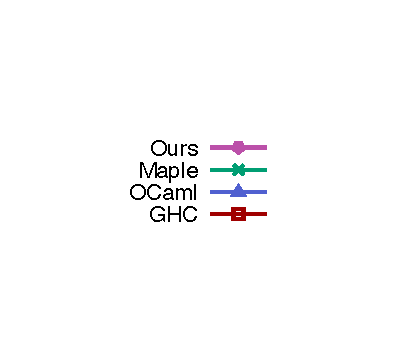
\includegraphics[scale=0.9]{figs/legend.pdf}
\end{subfigure}
%
\hspace{0.19\linewidth}
%
\begin{subfigure}[t]{0.3\linewidth}
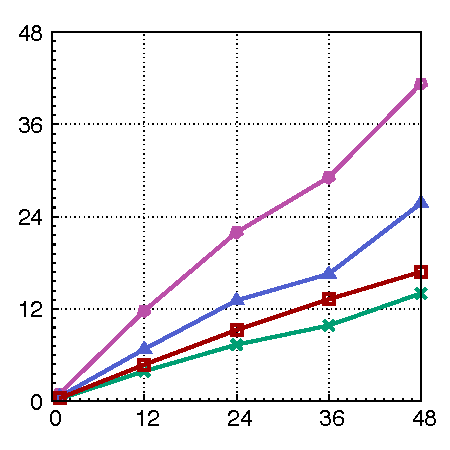
\includegraphics[scale=0.5]{figs/Fib.pdf}
\caption{fib}
\end{subfigure}
%
\hspace{0.01\linewidth}
%
\begin{subfigure}[t]{0.3\linewidth}
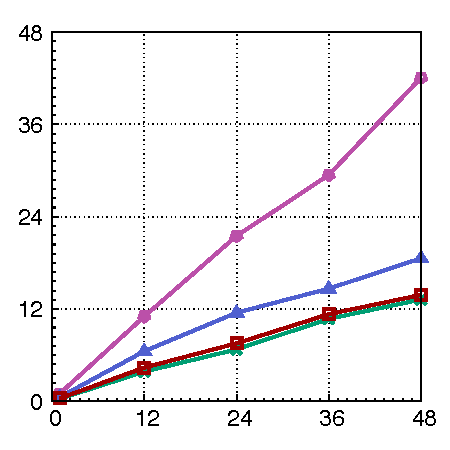
\includegraphics[scale=0.5]{figs/BuildFib.pdf}
\caption{buildtreeHvyLf}
\end{subfigure}
%
\\
\vspace{0.02\linewidth}
\hspace{0.04\linewidth}
%
\begin{subfigure}[t]{0.3\linewidth}
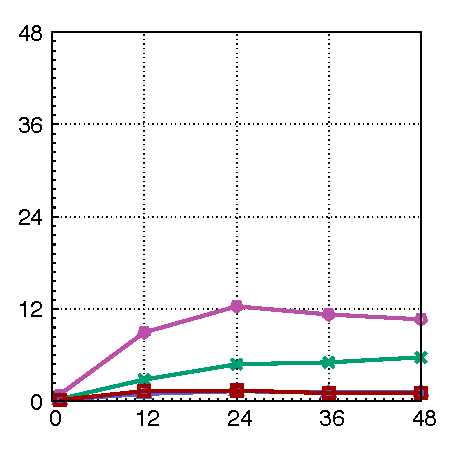
\includegraphics[scale=0.5]{figs/BuildKdTree.pdf}
\caption{buildKdTree}
\end{subfigure}
%
\hspace{0.005\linewidth}
%
\begin{subfigure}[t]{0.3\linewidth}
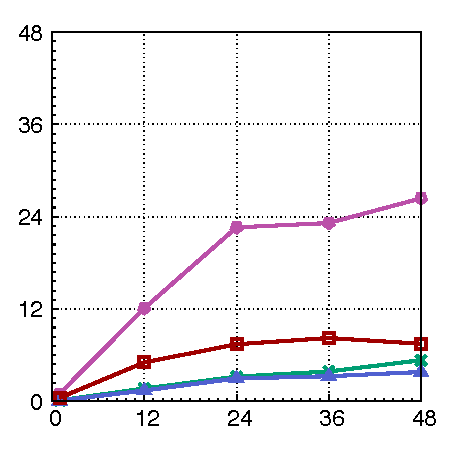
\includegraphics[scale=0.5]{figs/CountCorr.pdf}
\caption{countCorr}
\end{subfigure}
%
\hspace{0.02\linewidth}
%
\begin{subfigure}[t]{0.3\linewidth}
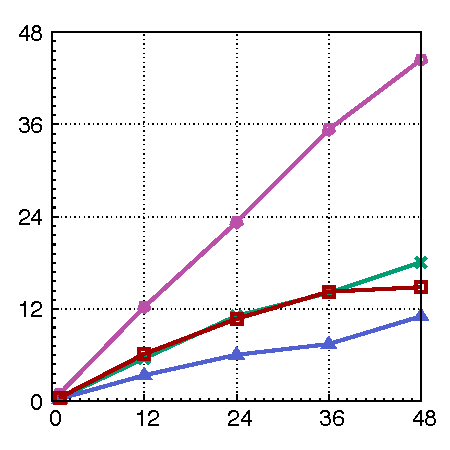
\includegraphics[scale=0.5]{figs/AllNearest.pdf}
\caption{allNearest}
\end{subfigure}
\\
\vspace{0.02\linewidth}
\hspace{0.03\linewidth}
%
\begin{subfigure}[t]{0.3\linewidth}
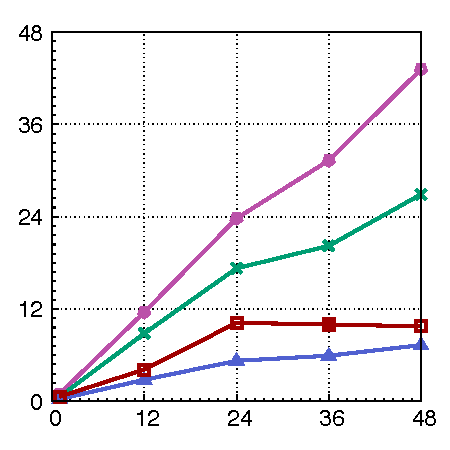
\includegraphics[scale=0.5]{figs/BarnesHut.pdf}
\caption{barnesHut}
\end{subfigure}
%
\hspace{0.022\linewidth}
%
\begin{subfigure}[t]{0.3\linewidth}
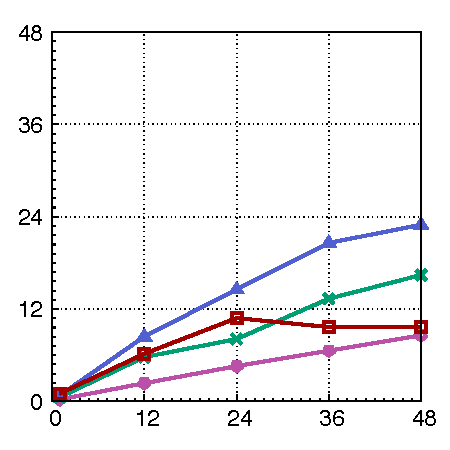
\includegraphics[scale=0.5]{figs/Coins.pdf}
\caption{coins}
\end{subfigure}
%
\hspace{0.005\linewidth}
%
\begin{subfigure}[t]{0.3\linewidth}
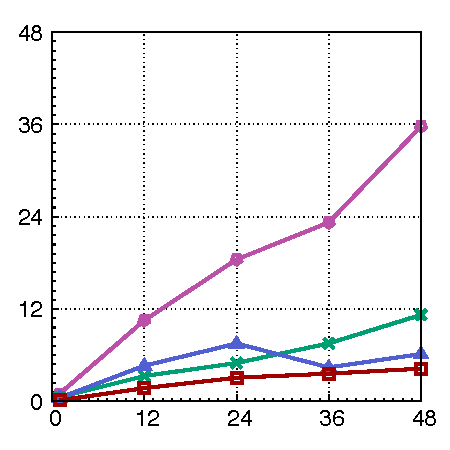
\includegraphics[scale=0.5]{figs/Countnodes.pdf}
\caption{countnodes}
\end{subfigure}
\\
\vspace{0.02\linewidth}
\hspace{0.05\linewidth}
%
\begin{subfigure}[t]{0.3\linewidth}
\includegraphics[scale=0.5]{figs/MergeSort.pdf}
\caption{mergeSort}
\end{subfigure}
%
\hspace{0.01\linewidth}
%
\begin{subfigure}[t]{0.3\linewidth}
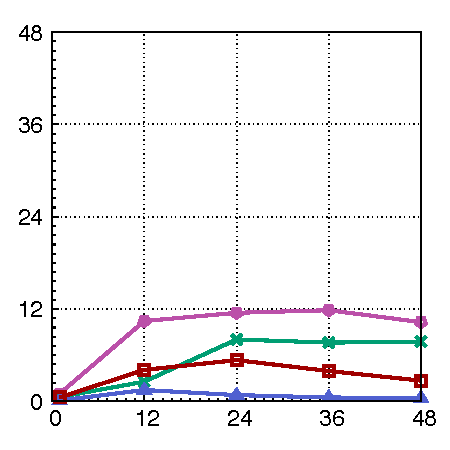
\includegraphics[scale=0.5]{figs/ConstantFolding.pdf}
\caption{constFold}
\end{subfigure}
%% %
\hspace{0.012\linewidth}
%
\begin{subfigure}[t]{0.3\linewidth}
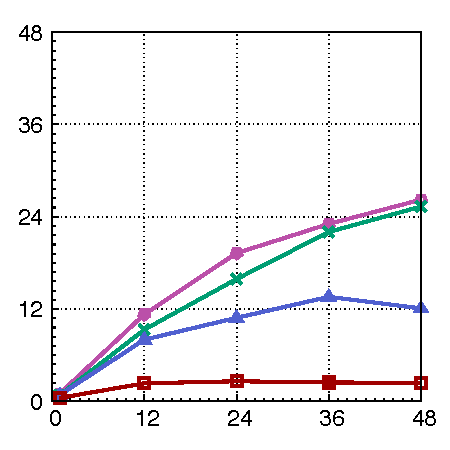
\includegraphics[scale=0.5]{figs/X86Compiler.pdf}
\caption{x86-compiler}
\end{subfigure}
\caption{
Speedups relative to the fastest sequential baseline, which is Sequential Gibbon
for all benchmarks except \il{coins}, in which case sequential GHC is fastest.
%% %
%% Note that Figure~(k) is scaled differently.
}
\label{fig:scaling-all}
\end{figure}
}

In \Secref{sec:evaluation}, we presented the results for \MPL{}, OCaml, and GHC
by showing speedups/slowdowns of our implementation relative to them.
%
In this section, we give the full evaluation results.
%
To make this section somewhat self-contained, we also include a copy of
Figure~\ref{fig:gibbon-table}, which compares the performance of sequential
and parallel Gibbon.
%
\Figref{fig:others-benchmark-results} shows the self-relative comparisions
for \MPL{}, OCaml and GHC.
%
The quantities in the table can be interpreted as follows.
%
Column $T_s$ shows the run-time of a sequential program,
which serves the purpose of a sequential baseline.
%
$T_1$ is the run-time of a parallel program on a single thread, and
$O$ the percentage overhead relative to $T_s$,
calculated as $((T_1 - T_s) / T_s) * 100$.
%
$T_{48}$ is the run-time of a parallel program on 48 threads and
$S$ is the speedup relative to $T_s$, calculated as $T_s / T_{48}$.
%
These comparisions are {\em self-relative}, meaning that they compare sequential \MPL{} to
parallel \MPL{}, sequential OCaml to parallel OCaml, and sequential GHC to parallel GHC.
%
With respect to self-relative comparisons,
on average, we scale similarly to \MPL{}, and {\em better} than OCaml or GHC,
and the single-thread overhead across all four compilers is comparable to each other.
%
\Figref{fig:scaling-all} shows speedups on 1-48 threads
relative to the fastest sequential baseline, which is Sequential Gibbon
for all benchmarks except \il{coins}, for which GHC is fastest.

\begin{figure}[h!]
  %% \setlength{\tabcolsep}{0.4em}
%% D{.}{.}{2.3}
\setlength{\tabcolsep}{0.3em}
\renewcommand{\arraystretch}{1.15}
\begin{tabular}{@{}l cc cccc@{}}
    \toprule
    & Gibbon & \phantom{} & \multicolumn{4}{c}{Ours} \\
    \cmidrule{2-2}
    \cmidrule{4-7}
    Benchmark & $T_s$ && $T_1$ & O & $T_{48}$ & S \\

    \midrule
    
    %% & (1) && (2) & (3) & (4) & (5) \\
    %% \midrule

    %%
    fib & 12.8 && 12.8 & 0 & 0.31 & 41.3 \\

    %%
    %% \buildfib{} & 4.6 && 4.61 & 0.22 & 0.11 & 41.8 \\
    \buildfib{} & 4.69 && 4.69 & 0 & 0.11 & 42.6 \\

    %% %% %%
    %% %% buildTree & 1.1 && 1.1 & & 0.17 & 6.5 \\

    %% %% %%
    %% %% add1Tree & 1.29 && 1.33 & & 0.15 & 8.6 \\

    %% %% %%
    %% %% sumTree & 0.32 && 0.32 & & 0.018 & 17.8 \\

    %% %%
    %% buildKdTree & 2.09 && 2.5 & 19.6 & 0.19 & 11 \\
    buildKdTree & 2.33 && 2.67 & 14.6 & 0.22 & 10.6 \\

    %%
    %% countCorr & 1.45  && 1.44 & -0.68 & 0.054 & 26.8 \\
    countCorr & 1.46  && 1.47 & 0.68 & 0.044 & 33.2 \\

    %%
    %% allNearest & 0.82 && 0.82 & 0 & 0.02 & 41 \\
    allNearest & 1.0 && 1.01 & 1 & 0.023 & 43.5 \\

    %% %% %%
    %% %% buildQuadTree & && & & & \\

    %% %%
    %% barnesHut(4M) & 14.43 && 14.42 & -0.069  & 0.35 & 40.9 \\

    %%
    %% barnesHut & 2.71 && 2.72 & 0.37  & 0.063 & 43 \\
    barnesHut & 3.21 && 3.21 & 0 & 0.074 & 43.4 \\

    %% %%
    %% %% buildBvh & && & & & \\

    %% %% %%
    %% %% ray & && & & & \\

    %%
    coins & 3.04 && 3.13 & 3 & 0.096 & 31.7 \\

    %%
    countnodes & 0.21 && 0.21 & 0 & 0.006 & 35.0 \\

    %%
    %% foldConstants & 1.71 && 1.71 & 0 & 0.17 & 10 \\
    constFold & 1.78 && 1.78 & 0 & 0.16 & 11.1 \\
    
    %% %% old, incorrect
    %% x86-compiler & 0.053 && 0.056 & 5.6 & 0.018 & 2.94 & 123 \\

    %% %% correct, big input
    %% x86-compiler & 5.98 && 5.98 & 0 & 0.16 & 37.4  & -  \\

    %% correct, small input
    x86-compiler & 1.08 && 1.08 & 0 & 0.041 & 26.3 \\

    %%
    %% mergeSort & 1.65 && 1.64 & -0.71 & 0.043 & 38.4 \\
    mergeSort & 1.58 && 1.60 & 1.27 & 0.039 & 40.5 \\

\iftoggle{isappendix}{
\midrule
average & - && - & 1.28 & - & 29.5 \\
}{
}
    \bottomrule
\end{tabular}

  \caption{
  A copy of \Figref{fig:gibbon-table} which compares performance of
  sequential and parallel Gibbon.
  }
\end{figure}

\begin{figure}[h!]
  %% \renewcommand{\arraystretch}{1.3}
  \setlength{\tabcolsep}{0.4em}
  \setlength{\tabcolsep}{0.14em}
\renewcommand{\arraystretch}{1.2}
\begin{tabular}{@{}l ccccc r ccccc r ccccc@{}}
    \toprule
    & \multicolumn{5}{c}{\MPL{}} & \phantom{} & \multicolumn{5}{c}{OCaml} & \phantom{} & \multicolumn{5}{c}{GHC} \\
    \cmidrule{2-6}
    \cmidrule{8-12}
    \cmidrule{14-18}
    Benchmark & $T_s$ & $T_1$ & O & $T_{48}$ & S && $T_s$ & $T_1$ & O & $T_{48}$ & S && $T_s$ & $T_1$ & O & $T_{48}$ & S \\
    \midrule

    %% & (1) & (2) & (3) & (4) & (5) && (6) & (7) & (8) & (9) & (10) && (11) & (12) & (13) & (14) & (15) \\
    %% \midrule

   %%
   %% fib & 46.03 & 46.3 & 0.58 & 1.06  & 43.4  && 21.1  & 21.12  & 0.09 & 0.5  & 42.2  && 31.88  & 31.84  & -0.12  & 0.76 & 41.9  \\
   fib & 37.4 & 38.6 & 3.2 & 0.91 & 41.1 && 21.1  & 21.1  & 0 & 0.5  & 42.2 && 31.9  & 31.8  & -0.3 & 0.76 & 42  \\

   %%
   %%  \buildfib{} & 18.36 & 18.22  & -0.76 & 0.44  & 41.7  && 7.73  & 7.73  & 0 & 0.185  & 41.8  && 11.76  & 11.77  & 0.1  & 0.34 & 34.6  \\
    \buildfib{} & 14.5 & 14.6 & 0.69 & 0.35 & 41.4 && 8.6 & 8.6 & 0 & 0.25 & 34.4 && 12.4 & 12.4 & 0 & 0.34 & 36.5  \\

   %%  %% %%
   %%  %% buildTree & 1.13  & 1.82  &  & 0.2  & 5.7  && 5.99  & 6.01  &  & 1.88  & 3.3  && 3.76  & 3.87  &  & 1.55  & 2.4 \\

   %%  %% %%
   %%  %% add1Tree & 2.63  & 3.6  &  & 0.38  & 6.9  && 9.84  & 9.78  &  & 2.99  & 3.3  && 4.13  & 4.08  &  & 1.82  & 2.3  \\

   %%  %% %%
   %%  %% sumTree & 1.51  & 1.54  &   & 0.06  & 25.2  && 0.42 & 0.42  &  & 0.021  & 20 && 0.62 & 0.63  &  & 0.052  & 11.9  \\

   %%
   %%  buildKdTree & 6.92  & 9.21 & 33.1  & 0.31  & 22.3  && 11.05 & 12.06 & 9.14  & 1.65 & 6.7 && 13.09 & 13.17 & 0.6 & 0.62 & 21.1 \\
   buildKdTree & 7.26 & 7.65 & 5.37 & 0.41 & 17.7 && 10.9  & 11.7  & 7.34 & 1.84 & 5.92 && 13.4  & 13.6 & 1.5 & 2.21 & 6.06  \\

    %%
    %% countCorr & 9.09  & 9.05 & -0.44  & 0.27  & 33.7  && 13.38 & 13.72 & 2.54  & 0.3 & 44.6  && 2.9 & 2.92 & 0.7  & 0.14 & 20.7  \\
    countCorr & 10.5 & 10.5 & 0 & 0.27 & 38.9  && 13.9 & 15.0 & 7.9 & 0.37 & 37.6 && 3.54 & 3.57 & 0.84 & 0.15 & 23.6 \\

    %%
    %% allNearest & 1.89 & 1.89  & 0  & 0.05  & 37.8  && 2.42 & 2.84 & 17.3 & 0.082 & 29.5  && 1.28  & 1.47 & 14.8 & 0.048 & 26.7  \\
    allNearest & 2.38 & 2.4 & 0.84 & 0.06 & 39.6 && 3.01 & 3.09 & 2.65 & 0.091 & 33.1 && 2.07  & 2.04 & -1.4 & 0.068 & 30.4  \\

   %%  %% %%
   %%  %% buildQuadTree &  &  &  &  &  &&  &  &  &  &  &&  &  &  &  &  \\

    %%
    %% barnesHut & 4.74  & 4.78  & 0.84  & 0.117  & 40.5 &&  9.22  & 9.1  & -1.3 & 0.36  & 25.6  && 4.62 & 5.53  & 19.7  & 0.36  & 12.8  \\
    barnesHut & 5.05  & 5.33 & 5.5 & 0.12 & 42 && 10.9 & 11 & 0.91 & 0.44 & 24.7 && 4.97 & 5.29 & 6.4 & 0.33 & 15.1  \\

   %%  %% %%
   %%  %% buildBvh &  &  &  &  &  &&  &  &  &  &  &&  &  &  &  &  \\

   %%  %% %%
   %%  %% ray &  &  &  &  &  &&  &  &  &  &  &&  &  &  &  &  \\

    %%
    coins & 1.71 & 1.51  & -11\% & 0.05 & 34.2 && 1.05  & 1.07  & 1.9  & 0.036  & 29.1  && 0.82 & 0.82 & 0  & 0.085  & 9.6  \\

    %%
    countnodes & 0.37  & 0.38  & 2.7 & 0.019 & 19.5  && 0.46 & 0.45  & -2.17  & 0.034 & 13.5  && 1.45 & 1.46 & 0.68  & 0.049 & 29.6  \\

    %%
    %% foldConstants & 2.31  & 3.03  & 31.1  & 0.22 & 10.5  && 14.8  & 15.8  & 6.75 & 3.84 & 3.85  && 3.43 & 3.34 & \Red{-2.6} & 0.63 & 5.44  \\
    constFold & 2.36  & 3.29  & 39.4 & 0.23 & 10.3 && 17.7 & 19.2 & 8.5 & 2.23 & 7.94 && 3.71 & 3.99 & 7.55 & 0.64 & 5.80 \\

    
    %% old, incorrect
    %% x86-compiler & 0.082 & 0.086 & 4.87 & 0.037 & 2.22 && 0.22 & 0.23 & 4.54 & 0.13 & 1.74 && 0.058 & 0.063 & 8.62 & 0.03 & 1.93 \\

    %% %% correct, big input
    %% x86-compiler & 8.09 & 8.08 & -0.12 & 0.2 & 40.4 && 6.9 & 7.28 & 5.5  & 0.25  & 27.6  && 13.9 & 13.9 & 0 & 1.25 & 11.1  \\

    %% correct, small input
    x86-compiler & 1.34 & 1.33 & -0.74 & 0.042 & 31.9 && 1.2  & 1.3 & 8.33 & 0.09 & 13.3  && 2.34 & 2.38  & 1.7  & 0.44 & 5.31  \\

    %% %%
    %% x86-compiler* & 4.01 & 4.33 & 7.98 & 1.39 & 2.88 && - & - & - & - & - && 2.5 & 2.76 & 10.4 & 1.3 & 1.92 \\

    %%
    %% mergeSort & 1.6 & 1.75 & 9.4 & 0.047 & 34  && 3.88 & 3.98  & 2.63 & 0.2 & 19.4  && 2.93 & 3.19 & 8.8 & 0.17 & 17.2 \\
    mergeSort & 1.74 & 1.84 & 5.75 & 0.048 & 36.3 && 3.83  & 3.94  & 2.87 & 0.19 & 20.16 && 2.74  & 2.95 & 7.66 & 0.16 & 17.1  \\

   \midrule
    average & - & - & 3.29 & - & 33.7  && - & - & 4.14 & - & 15.3 && - & - & 1.35 & - & 15.2 \\

    \bottomrule
  \end{tabular}
  
  \caption{
    Execution time in seconds,
    self-relative overheads on a single thread (Columns 3, 8 and 13)
    and self-relative speedups on 48 threads (Columns 5, 10 and 15).
    %
    $T_s$ is the run-time of a sequential program.
    %
    %% Columns
    $T_1$ and $T_{48}$ are the run-times of a parallel program
    on 1 thread and on 48 threads respectively.
    %
    $O$ is the single-thread percentage overhead: $O = (T_1 - T_s) / T_s * 100$.
    %
    $S$ is the 48-thread speedup: $S = T_s / T_{48}$.
  }
  \label{fig:others-benchmark-results}
\end{figure}



\section{Appendix: Formalism}
\label{sec:appendix-formalism}

This section contains:
\begin{enumerate*}[label*=(\arabic*)]
\item typing rules for \ourcalc{} (\Secref{subsec:appendix-typing-rules}),
\item a complete version of the dynamic semantics (\Secref{subsec:appendix-dynamic-semantics}),
\item definitions of all metafunctions used in the formalism (\Secref{subsec:appendix-metafunctions}),
\item well-formedness judgments for various elements of the formal model (\Secref{subsec:well-formedness-judgments}),
\item and the complete proof of type-safety for
\rparcalc{} (\Secref{subsec:appendix-type-safety}).
\end{enumerate*}

\subsection{Typing rules for \ourcalc{}}
\label{subsec:appendix-typing-rules}

Our type system for \rparcalc{} requires some substantial extensions
to the original type system given by \citet{LoCal}.
%
These extensions address the need to handle multi-task configurations,
which require a number of new typing environments and rules.
%
Before we present these extensions, we recall the typing rule
for the configuration of a single task, which is mostly unchanged from
the original.
%
\[ \TENV;\SENV;\CENV;\AENV;\NENV \vdash \AENV'; \NENV'; \EXPR : \hTYP \]
%
The context for this judgement includes five different environments. 
First, $\TENV$ is a standard typing environment.
Second, $\SENV$ is a store-typing environment, mapping 
\emph{materialized} symbolic locations to their types. That is, every location in $\SENV$ {\em has been written} and contains a value of type $\SENV(l^r)$.
Third, $\CENV$ is a constraint environment, keeping
track of how symbolic locations relate to each other.
Fourth, $\AENV$ maps each region in scope to a location, and is used to symbolically
track the allocation and incremental construction of data structures;
%% $\AENV$ can be thought of as representing the
%% \emph{focus} within a region of the computation.
% (the exact usage of $\AENV$ will be expanded on below).
Finally, $\NENV$ is a nursery of all symbolic locations that have been allocated,
but not yet written to.
%% Locations are removed from $\NENV$
%% upon being written to, as the purpose is to prevent multiple writes to
%% a location.
Both $\AENV$ and $\NENV$ are threaded through the typing
rules, also occuring in the output of the judgement, to the right of the
turnstile.

{
\small
\begin{figure}[h!]
\begin{mathpar}
\rtdataconivars{}
\end{mathpar}
\caption{An additional typing rule for type checking an in-flight data constructor.}
\label{fig:tdatacon-ivars}
\end{figure}
}

Let us first consider the rule \textsc{\tdatacon} given in \Figref{fig:static-semantics}.
%
It starts by ensuring that the tag being written, and all the fields have the
correct type.
%
Along with that, the locations of all the fields of the constructor must
also match the expected constraints.
%
That is, the location of the first field
should be immediately after the constructor tag, and there should be
appropriate $\mathit{after}$ constraints for other fields in the
location constraint environment.
%
To indicate that the tag has been written, the allocation environment is extended,
and the location $\loc$ is removed from the nursery,
to prevent multiple writes to a location.
%
However, if any fields of the constructor have evaluated to an \il{ivar},
the tag {\em is not} written to the store (\dregpardataconjoin{}).
%
The rule \textsc{\tdataconivars{}} handles this case.
%
It does not extend the allocation environment, and also keeps the location $\loc$
in the nursery, so that a constructor tag may be written at this location
in the future, once this task has synchronized with those
allocating the fields.
%
This additional typing rule is necessary to satisfy a requirement of
the Top Level Preservation lemma (\ref{lemma:preservation}).

To generalize our typing rules to handle multi-task configurations, we
introduce new environments for variables $\TENVMAP$, store
typing $\SENVMAP$, allocation constraints $\CENVMAP$, allocation
pointers $\AENVMAP$, and nurseries $\NENVMAP$.
%
These environments extend their counterparts in the sequential
\seqcalc{} type system, and are needed to track state on a per-task
basis.
%
The precise typing rules to type check a parallel task $\TASKVAR$, and
a set of parallel tasks $\TASKSET$ are given in
the \Figref{fig:appendix-static-semantics-parallel}.
%
A parallel task $\TASKVAR$ is well-typed if its target expression
$\EXPR$ is well-typed, using the original \seqcalc{} typing rules, and
a task set $\TASKSET$ is well-typed if all tasks in in it are
well-typed.

%
{
%% \floatstyle{boxed}\restylefloat{figure}
\begin{figure}
\begin{displaymath}
  \begin{aligned}
    \textup{Typing Env. Map} && \TENVMAP && \gramdef & \; \set{\concretelocvar_1 \mapsto \TENV_1, \; \ldots \; , \concretelocvar_n \mapsto \TENV_n} \\
    \textup{Store Typing Map} && \SENVMAP && \gramdef & \; \set{\concretelocvar_1 \mapsto \SENV_1, \; \ldots \; , \concretelocvar_n \mapsto \SENV_n} \\
    \textup{Constraint Env. Map} && \CENVMAP && \gramdef & \; \set{\concretelocvar_1 \mapsto \CENV_1, \; \ldots \; , \concretelocvar_n \mapsto \CENV_n} \\
    \textup{Allocation Pointers Map} && \AENVMAP && \gramdef & \; \set{\concretelocvar_1 \mapsto \AENV_1, \; \ldots \; , \concretelocvar_n \mapsto \AENV_n} \\
    \textup{Nursery Map} && \NENVMAP && \gramdef & \; \set{\concretelocvar_1 \mapsto \NENV_1, \; \ldots \; , \concretelocvar_n \mapsto \NENV_n}
  \end{aligned}
\end{displaymath}
\caption{Extended grammar of \ourcalc{} for static semantics.}
\label{fig:appendix-static-semantics-parallel-grammar}
\end{figure}
%% \floatstyle{plain}\restylefloat{figure}
}
%
%% \floatstyle{boxed}\restylefloat{figure}
{
\small      
\begin{figure}
\begin{mathpar}
%% \mprset{flushleft}
\rttask{}
\quad
\rttasksetempty{} \\
\rttaskset{}
\end{mathpar}
\caption{A copy of the typing rules given in \Figref{fig:static-semantics-parallel}.}
\label{fig:appendix-static-semantics-parallel}
\end{figure}
%% \floatstyle{plain}\restylefloat{figure}
}

{
\small
%% \floatstyle{boxed}\restylefloat{figure}
\begin{figure}[h!]
\begin{mathpar}
\mprset{flushleft}
\rtvar{}\quad\quad
\rtconcreteloc{}\\
\rtlet{}\quad\quad
\rtlregion{}\\
\rtllstart{}\\
\rtlltag{}\\
\rtllafter{}\\
\rtdatacon{}\quad\quad
\rtcase{}
\end{mathpar}
\caption{A copy of the typing rules for \seqcalc{} given in \cite{LoCal}}
\label{fig:static-semantics}
\end{figure}
%% \floatstyle{plain}\restylefloat{figure}
}

{
\small
%% \floatstyle{boxed}\restylefloat{figure}
\begin{figure}[h!]
\begin{mathpar}
\mprset{flushleft}
\rtapp{}\\\\
\rtfunctiondef{}\\\\
\rtpat{}\\\\
%% \rtcase{}
%% \quad
\rtprogram{}
\end{mathpar}
\caption{A copy of remaining typing rules for \seqcalc{} given in \cite{LoCal}}
\label{fig:static-semantics2}
\end{figure}
%% \floatstyle{plain}\restylefloat{figure}
}

\clearpage

\subsection{Dynamic semantics rules for \ourcalc{}}
\label{subsec:appendix-dynamic-semantics}

Figures~\ref{fig:dynamic-sequential-all} and~\ref{fig:dynamic-parallel-all} show
the complete dynamic semantics of \ourcalc{}.
%
These rules also appear in the main body of the paper,
but we include their copies here to make the appendix somewhat self-contained.
%
The driver which runs a \ourcalc{} program initially loads all data
types, functions, type checks them, and if successful, then seeds the
$Function$, $\typeofcon$, and $\typeoffield$ environments.
%
Let $\EXPR_0$ be the main expression.
%
If $\EXPR_0$ type checks with respect to the \tprogram{} rule, then
the main program is safe to run.
%
The initial configuration for the machine is a single task,
$\taskconfig{\hTYP}{\concreteloc{\reg}{0}{}}{\emptyset;\set{\loc \mapsto \concreteloc{\reg}{0}{}};\EXPR_0}$,
%
and the program can start taking evaluation steps from this initial configuration.
%
This configuration can be constructed automatically in a
straightforward way.

{
%% \floatstyle{boxed}\restylefloat{figure}
\small  
\begin{figure}[h!]
  \small
  \normalsize
  \begin{mathpar}
    \mprset{flushleft}
    \rdregparapp{}\quad\quad
    \rdregparletregion{}\\
    \rdregionparletloctag{}\\
    \rdregparletlocafterseq{}\quad\quad
    \rdregparletlocafternewreg{}\\
    \rdregionparletlocstart{}\quad
    \rdregionpardatacon{}\\
    \rdregparletexp{}\quad\quad
    \rdregparletval{}\\
    \rdcase{}
    %% \rregpardcase{}\\
  \end{mathpar}
  \caption{A complete version of dynamic semantics rules (sequential transitions).}
  \label{fig:dynamic-sequential-all}
\end{figure}
%% \floatstyle{plain}\restylefloat{figure}
}

{
%% \floatstyle{boxed}\restylefloat{figure}
\small  
\begin{figure}
  \small
  \normalsize
  \begin{mathpar}
    \mprset{flushleft}
    \rdregparsteptaskapp{}\\
    \rdregparletexpparapp{}\\
    \rdregparcasejoin\\
    \rdregpardataconjoin{}
  \end{mathpar}
  \caption{Copy of dynamic semantics rules (parallel transitions), given in \Figref{fig:dynamic-parallel}.}
  \label{fig:dynamic-parallel-all}
\end{figure}
%% \floatstyle{plain}\restylefloat{figure}
}

%% \clearpage
\subsection{Definitions of metafunctions}
\label{subsec:appendix-metafunctions}

In the following, we define various metafunctions used in our formal model.

\subsubsection{Merging task memories}
\label{subsec:appendix-merging-memories-region-parallel}

We merge two stores by merging the heaps of all the regions that are
shared in common by the two stores, and then by combining with all
regions that are not shared.
%
We merge two heaps by taking the set of the all the heap values at
indices that are equal, and all the heap values at
indices in only the first and only the second heap.
%
The merging of location maps follows a similar pattern, but is slightly
complicated by its handling of locations that map to ivars.
%
In particular, for any location where one of the two location maps
holds an ivar and the other one holds a concrete index, we assign
to the resulting location map the concrete index, because the concrete
index contains the more recent information.

{
%% \floatstyle{boxed}\restylefloat{figure}
\begin{figure}[h!]
\metafmerging
\caption{Metafunctions for merging task memories.}
\label{fig:appendix-merging-task-memories}
\end{figure}
%% \floatstyle{plain}\restylefloat{figure}
}

\subsubsection{End-Witness judgement}
\label{subsec:appendix-end-witness-judgement}

%% The end-witness rule is given in \Figref{fig:end-witness}.
%% %
The end-witness provides a naive computational interpretation
of the process for finding the index one past the end of a
given concrete location, with its given type.
%
This rule is mostly the same as the one given for the original, sequential \seqcalc{},
but includes an additional case for handling indirection pointers.
%
%% The end witness of a before index $\concreteloc{\reg}{\concretelocbefore{\svind{\ind}}}{}$
%% is simply $\concreteloc{\reg}{\svind{\ind}}{}$.
%% %
To compute the end-witness of an indirection pointer,
the judgement first reads the address $\concreteloc{\reg'}{\ind'_s}{}$ which is written
at $\concreteloc{\reg}{\ind_s}{}$,
and returns the end-witness of the value allocated at $\concreteloc{\reg'}{\ind'_s}{}$.

{
%% \floatstyle{boxed}\restylefloat{figure}
\begin{figure}[h!]
\noindent\paragraph{Case (A)} $\ewitness{\TYPC}{\concreteloc{\reg}{\concreteind{\ind_{s}}}{}}{\STOR}{\concreteloc{\reg}{\concreteind{\ind_{e}}}{}}$:

\begin{enumerate}%[label*=\arabic*]
\item \label{ewitness:impl1} $\STOR(\reg)(\ind_s) = \DC'$ \; \text{such that} \\
      $\; \DATA\;\TYPC = \overharpoon{\DC_1 \; \overharpoon{\sTYP}_1\;} \; | \; \ldots \; | \; \DC' \; \overharpoon{\sTYP}' \; | \; \ldots \; | \; \overharpoon{\DC_m \; \overharpoon{\sTYP}_m\;}$

\item \label{ewitness:impl4} $\overharpoon{\concreteind{w_0}} = \concreteind{\ind_s}+1$

\item \label{ewitness:impl2}
  $\ewitness{\overharpoon{\TYP'_1}}{\concreteloc{\reg}{\overharpoon{\concreteind{w_0}}}{}}{\STOR}{\concreteloc{\reg}{\overharpoon{\concreteind{w_1}}}{}} \wedge$ \\
  $\ewitness{\overharpoon{\TYP'_{j+1}}}{\concreteloc{\reg}{\overharpoon{\concreteind{w_j}}}{}}{\STOR}{\concreteloc{\reg}{\overharpoon{\concreteind{w_{j+1}}}}{}}$
  \\ where $\concreteind{\indj} \in \set{1,\ldots,n-1} ; n = | \overharpoon{\TYP'} |$

\item \label{ewitness:impl3}
  $\ind_e = \overharpoon{\concreteind{w_n}}$
\end{enumerate}

%% \noindent\paragraph{Case (B)} $\ewitness{\TYP}{\concreteloc{\reg}{\concretelocbefore{\svind{\ind}}}{}}{\STOR}{\concreteloc{\reg}{\svind{\ind}}{}}$

\noindent\paragraph{Case (B)} $\ewitness{\TYPC}{\concreteloc{\reg}{\concreteind{\ind_{s}}}{}}{\STOR}{\concreteloc{\reg'}{\concreteind{\ind'_{e}}}{}}$:

\begin{enumerate}%[label*=\arabic*]
%% \item  $\ind_e = \ind_s+1$

\item $\STOR(\reg)(\ind_s) = \indirection{\reg'}{\concreteind{\ind_s'}}$

\item $\ewitness{\TYPC}{\concreteloc{\reg'}{\concreteind{\ind_{s}'}}{}}{\STOR}{\concreteloc{\reg'}{\concreteind{\ind_{e}'}}{}}$
\end{enumerate}

\caption{The end-witness rule.}
\label{fig:end-witness}
\end{figure}
%% \floatstyle{plain}\restylefloat{figure}
}



\subsubsection{Linking fields of a data constructor}
\label{subsec:appendix-linking-fields}

%% In the region parallel execution model, the fields of a data constructor which
%% get computed in parallel with each other are allocated to separate regions.
%% %

Given a store $\STOR$, a location map $\MENV$, and the addresses of the
$n^{th}$ and $(n+1)^{th}$ fields of a data constructor $\DC$,
%% the metafunction $\tie$
this metafunction conditionally establishes a link between these fields.
%
If the location map $\MENV$ maps the symbolic location of the $(n+1)^{th}$ field,
$\locreg{\loc_2}{\reg_1}$, to an indirection pointer $\indirection{\reg_2}{\ind_2}$,
it means that these fields were computed in parallel with each other,
and thus would have been allocated into separate regions.
%
To link such fields, we use the end-witness judgement to compute an address
$\concreteloc{\reg_1}{\ind_e}{}$ which is one past the end of the $n^{th}$ field,
and we then write an indirection pointer pointing to the starting address of the $(n+1)^{th}$
field at $\concreteloc{\reg_1}{\ind_e}{}$.
%
This establishes the desired link.
%
If the fields have been allocated into the same region, we do not have to link them,
and the store $\STOR$ is returned unchanged in this case.
%
A precondition for using this metafunction is that the $n^{th}$ field must be fully
allocated.
%
%% The layout of the heap corresponding to different schedules
%% after establishing links between the fields is shown in \Figref{fig:datacon-layouts}.


{
%% \floatstyle{boxed}\restylefloat{figure}
\begin{figure}[h!]
\[
\begin{array}{lcl}
  \tie(\STOR,\MENV,\TYP_1,\concreteloc{\reg_1}{\concreteind{\ind_1}}{\loc_1}, \concretelocvar^{\loc_2}) = \STOR \cup \set{\reg_1 \mapsto (\concreteind{\ind_e} \mapsto \indirection{\reg_2}{\concreteind{\ind_2}})} \\  
  \text{where} \;\; (\locreg{\loc_2}{\reg_1} \mapsto \concreteloc{\reg_1}{\indirection{\reg_2}{\concreteind{\ind_2}}}{}) \in \MENV
  \; \text{and} \; \ewitness{\TYP_1}{\concreteloc{\reg_1}{\concreteind{\ind_1}}{}}{\STOR}{\concreteloc{\reg_1}{\concreteind{\ind_{e}}}{}}\\\\
  \tie(\STOR,\MENV,\TYP_1,\concreteloc{\reg_1}{\ind_1}{\loc_1}, \concretelocvar^{\loc_2}) = \STOR \\  
  \text{where} \;\; (\locreg{\loc_2}{\reg_1} \mapsto \concreteloc{\reg_1}{\indirection{\reg_2}{\concreteind{\ind_2}}}{}) \notin \MENV
\end{array}
\]
\caption{Metafunction for linking fields of a data constructor.}
\label{fig:appendix-linking-fields}
\end{figure}
%% \floatstyle{plain}\restylefloat{figure}
}


\subsubsection{Derefrencing indirections in $\MENV$}
\label{subsec:maplookup}

If a location $\loc$ maps to an indirection pointer $\indirection{\reg'}{\ind}$ in $\MENV$,
it is derefrenced by returning the address $\concreteloc{\reg'}{\ind}{}$.
%
Otherwise, the mapping contained in $\MENV$ is returned unchanged.


{
%% \floatstyle{boxed}\restylefloat{figure}
\begin{figure}[h!]
\[
\begin{array}{l}
\maplookupone{\MENV}{\loc} = \concreteloc{\reg}{\indbef{\indj}}{} \;\; \text{where}
\begin{array}{l}
(\loc \mapsto \concretelocvar) \in \MENV(\loc) \\
\concreteloc{\reg}{\indbef{\indj}}{} = \followinm(\MENV, \concretelocvar)
\end{array} \\\\
  %
\followinm(\MENV,\concreteloc{\reg}{\indirection{\reg'}{\concreteind{\ind}}}{}) = \concreteloc{\reg'}{\concreteind{\ind}}{} \\
%% \followinm(\MENV,\concreteloc{\reg}{\indbef{\ind}}{}) = \concreteloc{\reg}{\indbef{\ind}}{}
\followinm(\MENV,\concreteloc{\reg}{\concreteind{\ind}}{}) = \concreteloc{\reg}{\concreteind{\ind}}{} \\
\followinm(\MENV,\concreteloc{\reg}{\indivar{\ivarid}}{}) = \concreteloc{\reg}{\indivar{\ivarid}}{}
\end{array}
\]
\caption{}
\label{fig:maplookup}
\end{figure}
%% \floatstyle{plain}\restylefloat{figure}
}

\subsubsection{Other global environments and metafunctions}
\label{subsec:other-metafunctions}

\begin{itemize}
\item $Function(f)$: An environment that maps a function $f$ to its definition $\FD$.

\item $Freshen(\FD)$: A metafunction that freshens all bound variables in function definition
$\FD$ and returns the resulting function definition.

\item $TypeOfCon(\DC):$ An environment that maps a data constructor to its type.

\item $TypeOfField(\DC,i)$: A metafunction that returns the type of the \il{i}'th field
of data constructor $\DC$.

\item $ArgTysOfConstructor(\DC)$: An environment that maps a data constructor to its field types.

\item $\allocptr{\reg}{\STOR}$ = $\max(\set{-1} \cup \set{ \indj \; | \; {(\reg \mapsto (\indj \mapsto \DC)) \in \STOR}})$: A metafunction that returns the highest allocated address in the store,
or -1 if nothing has been allocated yet.

\item $\isval{\EXPR}$: A metafunction that checks if an expression is a value or not.

\item $Ivars(\EXPR)$: A metafunction that yields the set of ivars that occur in the term $\EXPR$.

\item $ \singlewriter{\TASKSET}{\hTYP}{\indivar{\ivarid}} =
|\set{\taskconfig{\hTYP}{\concreteloc{\reg}{\indivar{\ivarid}}{\loc}}{\STOR;\MENV;\EXPR} \; | \; \exists_{\STOR,\MENV,\EXPR} . \taskconfig{\hTYP}{\concreteloc{\reg}{\indivar{\ivarid}}{\loc}}{\STOR;\MENV;\EXPR} \in \TASKSET}| = 1
$ \\
%
A metafunction that checks if there is exactly one task $\TASKVAR \in \TASKSET$
which can supply a value of type $\hTYP$ for $\indivar{\ivarid}$.

\item \getwriter{\TASKSET}{\hTYP}{\indivar{\ivarid}}:
A metafunction that returns a unique task $\TASKVAR \in \TASKSET$
which can supply a value of type $\hTYP$ for $\indivar{\ivarid}$
if it exists, or returns -1 otherwise.

%% \taskconfig{\hTYP}{\concreteloc{\reg}{\indivar{\ivarid}}{\loc}}{\STOR;\MENV;\EXPR}

%% \item $\taskcomplete{\TASKVAR}$:
%% A metafunction that checks whether a task has evaluated to a value.

\item $\taskcomplete{\taskconfig{\hTYP}{\concretelocvar}{\STOR;\MENV;\EXPR}} = \isval{\EXPR}$:
A metafunction that checks whether a task has evaluated to a value.
%

%% \item $ProperHalt(\TASKSET)$: A metafunction that checks if 

\item $deepSupersetEqS(\SENVMAP_1, \SENVMAP_2) = \SENVMAP_1 \supseteq \SENVMAP_2 \vee
( (\concretelocvar \mapsto \SENV_2) \in \SENVMAP_2 \Rightarrow
  (\concretelocvar \mapsto \SENV_1) \in \SENVMAP_1 \wedge \SENV_1 \supseteq \SENV_2
)
$:
A metafunction that checks if the first argument is a {\em deep} superset of the second.
%
In other words, the first argument can contain a mapping $(\concretelocvar \mapsto \SENV)$
which is not present in the second one and thus be a super set at the outer level.
%
Or a specific mapping within the first argument can be a super set of the corresponding
mapping within the second, and be a super set at an inner level.
%
Note that it uses an inclusive-or, and both these conditions may be simultaneously true.

\item $deepSupersetEqC(\CENVMAP_1, \CENVMAP_2)$:
A metafunction identical to $deepSupersetEqS$, but for $\CENVMAP$.

\item $a \xor b = (a \wedge \neg b) \vee (\neg a \wedge b)$:
A metafunction for the exclusive-or logical operator.

\end{itemize}

\subsection{Well-formedness judgments}
\label{subsec:well-formedness-judgments}

In this section we present certain well-formedness criteria for
various elements of the formal model.
%
Some of these are similar to the corresponding judgments for sequential \seqcalc{} given
in \cite{LoCal},
but they are extended to handle ivars, and indirections in the location map and store.
%
We give an additional judgement to check the well-formedness of the set of
tasks executing in a parallel machine.
%
Because there are many requirements specified inside the various
well-formedness judgments, we introduce notation for referring
to requirements individually.
%
For example, the notation
\refwellformed{sec:well-formedness-allocation}{wf:impl-linear-alloc2}
refers to the judgement
%% \begin{align*}
$\storewfca{\AENV}{\NENV}{}{\MENV}{\STOR}$,
%% \end{align*}
specified in Section~\ref{sec:well-formedness-allocation},
and in that judgement, rule number~\ref{wf:impl-linear-alloc2}.

\subsubsection{Well-formedness of a task set}
\label{sec:well-formedness-tasks}

This judgement specifies certain invariants that should hold
for all tasks executing in a parallel machine
for the task set to be well-formed.
%
Rule~\ref{wf:ivar-present} specifies that for all ivars referenced in an
expression being computed by a certain task,
%
there is a corresponding ivar in the location map,
%
and there is exactly one other task in the task set which supplies a
well-typed value for that ivar.
%% %
%% Rule~\ref{wf:region-parallel-invariant-store} specifies that the stores of two separate tasks
%% can share no common regions, which is a way of establishing the region-parallel invariant ---
%% only a single task may allocate to a certain region at a time.
%
Rule~\ref{wf:task-store-wf} references a separate judgement for well-formedness of the
store with respect to the location map of a parallel task.

\paragraph{Judgement form}

$\SENVMAP;\CENVMAP;\AENVMAP;\NENVMAP \storewftasks{\TASKSET}$

\paragraph{Definition}

% Dummy paragraph to force a newline
\paragraph{}

$\forall \taskconfig{\hTYP}{\concretelocvar{}}{\STOR;\MENV;\EXPR} \in \TASKSET.$

$
\SENV = \SENVMAP(\concretelocvar) ; \;
\CENV = \CENVMAP(\concretelocvar) ; \;
\AENV = \AENVMAP(\concretelocvar) ; \;
\NENV = \NENVMAP(\concretelocvar)
$

\begin{enumerate}
\item \label{wf:ivar-present} $
\concreteloc{\reg}{\indivar{\ivarid}}{\loc} \in Ivars(\EXPR) \wedge
 \emptyset;\SENV;\CENV;\AENV;\NENV \vdash \AENV' ; \NENV' ; \concreteloc{\reg}{\indivar{\ivarid}}{\loc} : \hTYP' \Rightarrow\\
 (\locreg{\loc}{\reg} \mapsto \concreteloc{\reg}{\indivar{\ivarid}}{\loc}) \in \MENV \wedge
 \singlewriter{\TASKSET}{\hTYP'}{\indivar{\ivarid}}
 $
 
%% \item \label{wf:region-parallel-invariant-store} $
%% \taskconfig{\hTYP'}{\concretelocvar{}'}{\STOR';\MENV';\EXPR'} \in \TASKSET
%% \Rightarrow
%% dom(\STOR) \cap dom(\STOR') = \emptyset$

\item \label{wf:task-store-wf} $\storewf{\SENV}{\CENV}{\AENV}{\NENV}{\TASKSET}{\MENV}{\STOR}$
\end{enumerate}

\subsubsection{Well-formedness of a store}
\label{sec:well-formedness}

\paragraph{Judgement form}

$\storewf{\SENV}{\CENV}{\AENV}{\NENV}{\TASKSET}{\MENV}{\STOR}$

The well-formedness judgement for a parallel task's
store specifies the valid layouts of the store by using the location
map and the various environments from the typing judgement.
%% %
%% This judgement is used by \ref{sec:well-formedness-tasks} to check the 
%
Rule~\ref{wf:map-store-consistency} specifies that, for each location $\locreg{\loc}{\reg}$
in the store-typing environment,
there is a corresponding address in the location map.
%
There are two possible ways in which the value at location $\locreg{\loc}{\reg}$
may be allocated --- (1) sequentially, by the current task, or
(2) in parallel, by a different task.
%
The first disjunct holds when the value is allocated sequentially by the current task.
%
In this case, the address in the location map is a concrete index, 
and it satisfies a corresponding end-witness judgement.
%
Otherwise, the second disjunct holds.
%
In this case, the address is an ivar,
there is exactly one task which allocates a value at this ivar,
its location map contains a concrete index as location $\locreg{\loc}{\reg}$'s address,
and if it has evaluated to a value, the concrete index satisfies
a corresponding end-witness judgement.
%
Note that these disjuncts are connected with an {\em exclusive-or}, and only of them
can hold at a time.
%
%% Alternatively, this address can be an ivar,
%% which means that the value at location $\locreg{\loc}{\reg}$
%% is allocated in parallel by a different task.
%% %
%
Rules~\ref{wf:cfc} and~\ref{wf:ca} reference the judgments for well-formedness concerning
in-flight constructor applications (\Secref{sec:well-formedness-constructors}) and correct allocation in
regions (\Secref{sec:well-formedness-allocation}), respectively.
%
Finally, Rule~\ref{wf:impl1} specifies that the nursery and store-typing environments reference
no common locations, which is a way of reflecting that each location is either in the process
of being constructed and in the nursery, or allocated and in the store-typing environment, but
never both.


\newcommand{\mapstoreconsistency}{
\ensuremath{
(\locreg{\loc}{\reg} \mapsto \TYP) \in \SENV \Rightarrow \\
            (\concreteloc{\reg}{\ind_1}{} = \hat{\MENV}(\locreg{\loc}{\reg}) \wedge
            \ewitness{\TYP}{\concreteloc{\reg}{\ind_1}{}}{\STOR}{\concreteloc{\reg}{\ind_2}{}}) \xor \\
            (\concreteloc{\reg}{\indivar{\ivarid}}{} = \hat{\MENV}(\locreg{\loc}{\reg}) \wedge
             \exists_{\STOR',\MENV',\EXPR'}. \taskconfig{\TYP}{\concreteloc{\reg}{\indivar{\ivarid}}{}}{\STOR';\MENV';\EXPR'} = \getwriter{\TASKSET}{\hTYP}{\indivar{\ivarid}} \wedge
             \concreteloc{\reg}{\ind_1}{} = \hat{\MENV'}(\locreg{\loc}{\reg}) \wedge \\
             (\isval{\EXPR'} \Rightarrow \ewitness{\TYP}{\concreteloc{\reg}{\ind_1}{}}{\STOR'}{\concreteloc{\reg}{\ind_2}{}})
             )
}}

\paragraph{Definition}

\begin{enumerate}%[label*=\arabic*]

    \item \label{wf:map-store-consistency} $\mapstoreconsistency{}$ 

    \item \label{wf:cfc} $\storewfcfa{\CENV}{}{\MENV}{\STOR}$

    \item \label{wf:ca} $\storewfca{\AENV}{\NENV}{}{\MENV}{\STOR}$

    \item \label{wf:impl1} $dom(\SENV) \cap \NENV = \emptyset $

\end{enumerate}

\subsubsection{Well-formedness of constructor application}
\label{sec:well-formedness-constructors}

\paragraph{Judgement form}

$\storewfcfa{\CENV}{}{\MENV}{\STOR}$

The well-formedness judgement for constructor application specifies the various constraints
that are necessary for ensuring correct formation of constructors, dealing with constructor
application being an incremental process that spans multiple \ourcalc{} instructions.
%
Rule~\ref{wfconstr:constraint-start} specifies that, if a location corresponding to the
first address in a region is in the constraint environment, then there is a corresponding
entry for that location in the location map.
%
Rule~\ref{wfconstr:constraint-tag} specifies that, if a location corresponding to the address one past a constructor
tag is in the constraint environment, then there are corresponding locations for the address
of the tag and the address after it in the location map.
%
Rule~\ref{wfconstr:constraint-after} specifies that, if a location corresponding to the address
one past after a fully allocated constructor application is in the constraint environment,
then there are corresponding locations
for the address of the start of that constructor application, and
for the address one past the constructor application in the location map.
%
There are two possible ways in which the values at locations $\locreg{\loc'}{\reg}$
and $\locreg{\loc}{\reg}$ may be allocated ---
(1) sequentially, by a single task, and thus in a single region, or
(2) in parallel with each other, by separate tasks, and thus in separate regions.
%
The first disjunct holds when the values are allocated sequentially by a single task.
%
In this case, the starting address of the constructor application is a concrete index,
and an end-witness for it also exists.
%
The address one past the constructor application is this end-witness.
%
The second disjunct holds when the values are allocated in parallel by separate tasks.
%
In this case, the location map $\MENV$ and store $\STOR$ belong to the task
that allocates the value at location $\locreg{\loc}{\reg}$.
%
The starting address of the constructor application is an ivar,
and the address one past the constructor application is an indirection pointer
pointing to a separate region which has been allocated in the store.
%
The third disjunct holds when the values are allocated in parallel by separate tasks,
but after those tasks have synchronized with each other, and their memories merged
(\ref{subsec:appendix-merging-memories-region-parallel}).
%
The merge resets the starting address of the constructor application back to
a concrete index, and an end-witness for it now exists.
%
The store contains an indirection pointer at this end-witness which points
to the start of the region that contains the value at location $\locreg{\loc}{\reg}$.
%
In other words, a link between the values at locations $\locreg{\loc'}{\reg}$ and
$\locreg{\loc}{\reg}$ exists.
%
The address one past the constructor application is the corresponding indirection pointer.
%
Note that these disjuncts are connected with an {\em exclusive-or}, and only of them
can hold at a time.


\paragraph{Definition}

\newcommand{\wfconstrstart}{
\ensuremath{
(\locreg{\loc}{\reg} \mapsto \startr{\reg}) \in \CENV \Rightarrow
(\locreg{\loc}{\reg} \mapsto \concreteloc{\reg}{0}{}) \in \MENV 
}}

\newcommand{\wfconstrtag}{
\ensuremath{
\locreg{\loc}{\reg} \mapsto (\locreg{\loc'}{\reg} + 1)) \in \CENV \Rightarrow
\concreteloc{\reg}{\ind_l}{} = \hat{\MENV}(\locreg{\loc'}{\reg}) \wedge
\concreteloc{\reg}{\ind_l + 1}{} = \hat{\MENV}(\locreg{\loc}{\reg})
}}

\newcommand{\wfconstrafter}{
\ensuremath{
(\locreg{\loc}{\reg} \mapsto \afterl{\tyatlocreg{\TYP}{\loc'}{\reg}}) \in \CENV \Rightarrow \\            
            (\concreteloc{\reg}{\ind_1}{} = \hat{\MENV}(\locreg{\loc'}{\reg}) \wedge
            \ewitness{\TYP}{\concreteloc{\reg}{\ind_1}{}}{\STOR}{\concreteloc{\reg}{\ind_2}{}} \wedge
            \concreteloc{\reg}{\ind_2}{} = \hat{\MENV}(\locreg{\loc}{\reg}))
            \xor \\
            ( \concreteloc{\reg}{\indivar{\ivarid_1}}{} = \hat{\MENV}(\locreg{\loc'}{\reg}) \wedge
                  (\locreg{\loc}{\reg} \mapsto \concreteloc{\reg}{\indirection{\reg_2}{0}}{}) \in \MENV \wedge
                  \set{\reg_2 \mapsto \heap} \in \STOR)            
             \xor \\            
            (\concreteloc{\reg}{\ind_1}{} = \hat{\MENV}(\locreg{\loc'}{\reg}) \wedge
            \ewitness{\TYP}{\concreteloc{\reg}{\ind_1}{}}{\STOR}{\concreteloc{\reg}{\ind_2}{}} \wedge
              (\locreg{\loc}{\reg} \mapsto \concreteloc{\reg}{\indirection{\reg_2}{0}}{}) \in \MENV \wedge
                 \STOR(\reg)(\ind_2) = \indirection{\reg_2}{0}
                 )
}}

\begin{enumerate}%[label*=\arabic*]
    \item \label{wfconstr:constraint-start} $\wfconstrstart{}$

    \item \label{wfconstr:constraint-tag} $\wfconstrtag{}$

    \item \label{wfconstr:constraint-after} $\wfconstrafter{}$

\end{enumerate}

\subsubsection{Well-formedness concerning allocation}
\label{sec:well-formedness-allocation}

\paragraph{Judgement form}

$\storewfca{\AENV}{\NENV}{}{\MENV}{\STOR}$

The well-formedness judgement for safe allocation specifies the various properties
of the location map and store that enable continued safe allocation, avoiding in particular
overwriting cells, which could, if possible, invalidate overall type-safety.
%
Rule~\ref{wf:impl-linear-alloc} requires that, if a location $\locreg{\loc}{\reg}$ is in both the allocation
and nursery environments, i.e., that address represents an in-flight
constructor application, then there is a corresponding location in the location
map and the address of that location is the highest address in the store.
%
Alternatively, the value at location $\locreg{\loc}{\reg}$ is allocated in parallel by
a separate task, in a separate region,
and its address is the corresponding indirection pointer.
%
Rule~\ref{wf:impl-linear-alloc2} requires that, if there is an address in the allocation
environment and that address is fully allocated, then the address of that location is the
highest address in the store.
%
Rule~\ref{wf:impl-write-once} requires that, if there is an address in the nursery, then
there is a corresponding location in the location map, but nothing at the corresponding
address in the store.
%
Finally, Rule~\ref{wf:impl-empty-region} requires that, if there is a region that has been
created but for which nothing has yet been allocated, then there can be no addresses
for that region in the store.

\paragraph{Definition}

\begin{enumerate}%[label*=\arabic*]
    \item \label{wf:impl-linear-alloc} $ ((\reg \mapsto \locreg{\loc}{\reg}) \in \AENV \wedge \locreg{\loc}{\reg} \in \NENV) \Rightarrow \\
          ((\locreg{\loc}{\reg} \mapsto \concreteloc{\reg}{\ind}{}) \in \MENV \wedge
%          \ind = \max \set{0} \cup \set{\indj \; | \; \concreteloc{\reg}{\indj}{} \in \MENV} \wedge \\
          \ind > \allocptr{\reg}{\STOR})
          \xor
          (\locreg{\loc}{\reg} \mapsto \indirection{\reg_2}{\ind_2}) \in \MENV
          $

    \item \label{wf:impl-linear-alloc2} $ ((\reg \mapsto \locreg{\loc}{\reg}) \in \AENV \wedge 
    \, \concreteloc{\reg}{\ind_s}{} = \hat{\MENV}(\locreg{\loc}{\reg}) \wedge
    \locreg{\loc}{\reg} \not \in \NENV \wedge
    \, \ewitness{\TYP}{\concreteloc{\reg}{\ind_s}{}}{\STOR}{\concreteloc{\reg}{\ind_e}{}}) \Rightarrow
          \ind_e > \allocptr{\reg}{\STOR}
          $

    \item \label{wf:impl-write-once} $ \locreg{\loc}{\reg} \in \NENV \Rightarrow
          \concreteloc{\reg}{\ind}{} = \hat{\MENV}(\locreg{\loc}{\reg}) \wedge
          (\reg \mapsto (\ind \mapsto \DC)) \not \in \STOR
          $

    \item \label{wf:impl-empty-region} $(\reg \mapsto \emptyset) \in \AENV \Rightarrow
    (\reg \mapsto \emptyset) \in \STOR$
\end{enumerate}



\subsection{Type-Safety}
\label{subsec:appendix-type-safety}


We state the type-safety theorem as follows:
%
\begin{theorem}[Type Safety]
  \label{theorem:type-safety}
  \begin{displaymath}
  \begin{aligned}
  \text{If} \;\; & \emptyset;\SENVMAP;\CENVMAP;\AENVMAP;\NENVMAP \vdash_{taskset} \AENVMAP' ; \NENVMAP' ; \TASKSET \; \wedge \; \SENVMAP;\CENVMAP;\AENVMAP;\NENVMAP \storewftasks{\TASKSET} \\
  %% \text{and} \;\; &  \\
  \text{and} \;\; & \TASKSET \rparstepsto^{n} \TASKSET' \\
  \text{then, either} \;\; & \forall \TASKVAR \in \TASKSET'. \; \taskcomplete{\TASKVAR} \\
  \text{or} \;\; & \exists \; \TASKSET''. \; \TASKSET' \rparstepsto \TASKSET''.
  \end{aligned}
  \end{displaymath}
\end{theorem}
%
This theorem states that, if a given task set $\TASKSET$ is well typed
and its overall store is well formed, and if $\TASKSET$
%% can
makes a transition to some task set $\TASKSET'$ in $n$ steps,
then either all tasks in
$\TASKSET'$ are fully evaluated or $\TASKSET'$ can take
a step to some task set $\TASKSET''$.
%
As usual, we prove this theorem by showing progress and preservation.


\begin{lemma}[Top Level Progress]
  \label{lemma:single-task-progress}
  \begin{displaymath}
  \begin{aligned}
  \text{If} \;\; & \emptyset;\SENVMAP;\CENVMAP;\AENVMAP;\NENVMAP \tctaskset \AENVMAP' ; \NENVMAP' ; \TASKSET \\
  \text{and} \;\; & \SENVMAP;\CENVMAP;\AENVMAP;\NENVMAP \storewftasks{\TASKSET} \\
  \text{then} \;\; & \forall \TASKVAR \in \TASKSET.\; \taskcomplete{\TASKVAR} \\
  \text{else} \;\; & \TASKSET \rparstepsto \TASKSET'.
  \end{aligned}
  \end{displaymath}
\end{lemma}

\begin{bproof}

If every $\TASKVAR \in \TASKSET$ has evaluated to a value, we have no further
proof obligations.
%
Otherwise, the obligation is to show that there is at least one task which
can take a sequential or a parallel step.
%
By inversion on \ttaskset{}, and the typing rule given in the premise of this lemma,
we know that all tasks in the task set $\TASKSET$ are well-typed.
%
%% Thus, we need to show that there is at least one
%% well-typed task that has not evaluated to a value which can take a step.
%
Then, by inversion on \ttask{}, we know that the expression $\EXPR$
it is evaluating is also well-typed.
%
%% We show that a task evaluating a well-typed expression can take a step
We show that there is at least one $\TASKVAR \in \TASKSET$ which
can take a sequential or a parallel step,
%
by performing induction on the typing derivation of the expression $\EXPR$
that a task is evaluating.

\begin{bcase}[\tlet, $\; \EXPR = \letpack{\var : \hTYP_1}{\EXPR_1}{\EXPR_2}$]

\begin{mathpar}
\rtlet{}
\end{mathpar}

Because $\EXPR$ is not a value, the proof obligation is to show that there is at least one task which
can take a step. That is, there is a rule in the dynamic semantics whose
left-hand side matches the machine configuration $\TASKSET$.
%
There are two rules that can match.

\begin{enumerate}

\item
\begin{mathpar}
\mprset{flushleft}
\rdregparletexppar{}
\end{mathpar}


By inversion on \dregparletexppar{}, the only obligation is to estalish that
$\concretelocvar_1 = \hat{\MENV}(\locreg{\loc_1}{\reg_1})$.
%
%% By inversion on the well formedness of the task set given in the premise of this lemma,
%% we can apply the rule \refwellformed{sec:well-formedness-tasks}{wf:task-store-wf},
%
By applying the rule \refwellformed{sec:well-formedness-tasks}{wf:task-store-wf} for
the well-formedness of the task set given in the premise of this lemma,
we can obtain a well-formedness result for the store and location map used by this task:
$\storewf{\SENV}{\CENV}{\AENV}{\NENV}{\TASKSET}{\MENV}{\STOR}$.
%
%% By inversion on the well formedness of the task set given in the premise
%% of this lemma, we know that $\SENVMAP;\CENVMAP;\AENVMAP;\NENVMAP \storewftasks{\TASKSET}$.
%% %
%% By applying the rule \refwellformed{sec:well-formedness-tasks}{wf:task-store-wf},
%% we know that the store and the location map of this task are well formed:
%% $\storewf{\SENV}{\CENV}{\AENV}{\NENV}{\TASKSET}{\MENV}{\STOR}$.
%
We can then perform inversion on the well-formedness of the store,
and apply the rule \refwellformed{sec:well-formedness}{wf:ca} to obtain
$\storewfca{\AENV}{\NENV}{}{\MENV}{\STOR}$.
%
Finally, we apply \refwellformed{sec:well-formedness-allocation}{wf:impl-write-once}
to obtain $\concreteloc{\reg}{\ind}{} = \hat{\MENV}(\locreg{\loc_1}{\reg_1})$.
%
Thus we have discharged the proof obligation,
and this task can take a parallel step using \dregparletexppar{}.

\item
\begin{mathpar}
\mprset{flushleft}
\rdregparsteptask{}
\end{mathpar}

To obtain this result, we use Lemma~\ref{lemma:single-thread-progress}
for single thread progress.
%
There are two preconditions in order to use this lemma:
$\emptyset;\SENV;\CENV;\AENV;\NENV \vdash \AENV';\NENV';\EXPR : \hTYP$, and
$\storewf{\SENV}{\CENV}{\AENV}{\NENV}{\MENV}{\STOR}$.
%
The first precondition is already established at the start of the proof,
by performing inversion on \ttaskset{}, and then on \ttask{}.
%
The second precondition can be discharged
%% in a similar way as the previous case ---
%% by using similar reasoning to the previous case ---
by performing inversion on the
on the well-formedness of the task set given in the premise
of this lemma, and then applying the rule
\refwellformed{sec:well-formedness-tasks}{wf:task-store-wf}.

\end{enumerate}

\end{bcase}


\begin{bcase}[\tdataconivars, $\;\EXPR = \datacon{\DC}{\keywd{\locreg{\loc}{\reg}}}{\overharpoon{\VAL}}$]

\begin{mathpar}
\rtdataconivars{}
\end{mathpar}

Because $\EXPR$ is not a value, the proof obligation is to show that there is a task which
can take a step. That is, there is a rule in the dynamic semantics whose
left-hand side matches the machine configuration $\TASKSET$.
%
There are a single rule that can match.

%% \begin{enumerate}

%% \item
\begin{mathpar}
\rdregpardataconjoin{}
\end{mathpar}

If any of the fields of the data constructor have evaluated to an ivar,
the only rule that can match is \dregpardataconjoin{}.
%
By inversion on \dregpardataconjoin{}, the only obligation then is to find a task $\TASKVAR_c$
which supplies a value of that ivar.
%
To obtain this result we perform inversion on the well-formedness of the task set given in the premise
of this lemma, and apply the rule \refwellformed{sec:well-formedness-tasks}{wf:ivar-present}.
%
Thus, we know that exactly one such task $\TASKVAR_c$ exists.
%
There are two possible states in which the task $\TASKVAR_c$ may be in ---
it may have evaluated its expression to a value, or not.
%
If the former is true, then the rule \dregpardataconjoin{} matches, and this task
can take a step.
%
Otherwise, the $\TASKVAR_c$, or one of its child tasks can take a step,
and thus this case.


%% \item
%% \begin{mathpar}
%% \mprset{flushleft}
%% \rdregparsteptask{}
%% \end{mathpar}

%
%% \item
%% \begin{mathpar}
%% \rddatacon{}
%% \end{mathpar}\\

%% To obtain this result, we use Lemma~\ref{lemma:single-thread-progress}
%% for single thread progress like the previous case.

%% \end{enumerate}

\end{bcase}



\begin{bcase}[\tcase, $\;\EXPR = \case{\VAL}{\overharpoon{\pat} : \tyatlocreg{\TYP}{\loc}{\reg}}$]

Because $\EXPR$ is not a value, the proof obligation is to show that there is a task which
can take a step. That is, there is a rule in the dynamic semantics whose
left-hand side matches the machine configuration $\TASKSET$.
%
There are two rules that can match: \dregparcasejoin{}, or \dparsteptask{}.
%
With respect to \dregparcasejoin{}, it can can be discharged by using similar reasoning
as the \tdataconivars{} case.
%
As for \dparsteptask{}, we use Lemma~\ref{lemma:single-thread-progress}
for single thread progress like earlier.

\end{bcase}

\begin{bcase}

The cases for \tdatacon{}, \tlregion{}, \tlltag{}, \tllstart{}, \tllafter{}, \tvar{}, and \tconcreteloc{}
use the Lemma~\ref{lemma:single-thread-progress}
for single thread progress, and can be discharged by using similar reasoning to
the previous cases.

\end{bcase}

$\blacksquare$

\end{bproof}


\begin{lemma}[Single Thread Progress]
\label{lemma:single-thread-progress}
\begin{displaymath}
  \begin{aligned}
  \text{If} \;\; & \emptyset;\SENV;\CENV;\AENV;\NENV \vdash \AENV';\NENV';\EXPR : \hTYP \\
  \text{and} \;\; & \storewf{\SENV}{\CENV}{\AENV}{\NENV}{\MENV}{\STOR} \\
  \text{then} \;\; & \EXPR \; \mathit{value} \\
  \text{else} \;\; & \STOR;\MENV;\EXPR \stepsto \STOR';\MENV';\EXPR'.
  \end{aligned}
\end{displaymath}
\end{lemma}

\begin{bproof}

The proof is by induction on the typing derivation of $\EXPR$.

\begin{bcase}[\tllafter{}, $\; \EXPR = \letloc{\locreg{\loc}{\reg}}{\afterl{\tyatlocreg{\TYP'}{\loc_{1}}{\reg}}}{\EXPR'}$
]

\begin{mathpar}
\rtllafter{}
\end{mathpar}

Because $\EXPR$ is not a value, the proof obligation is to show that there is a task which
can take a step. That is, there is a rule in the dynamic semantics whose
left-hand side matches the machine configuration $\STOR;\MENV;\EXPR$.
%
There are two rules that can match: \dletlocafter{}, or
\dregparletlocafternewreg{}.
%
They both have a similar precondition: $\concretelocvar{} = \hat{\MENV}(\locreg{\loc_1}{\reg})$.
%
To obtain this result, we need to use
rule \refwellformed{sec:well-formedness}{wf:map-store-consistency}
of the well-formedness of the store given in the premise of this lemma.
%
This rule requires that $\SENV(\locreg{\loc_1}{\reg}) = \TYP'$,
which can be obtained by inversion on \tllafter{}.
%
By inversion on
\refwellformed{sec:well-formedness}{wf:map-store-consistency},
we can establish that either
$\concreteloc{\reg}{\ind}{} = \hat{\MENV}(\locreg{\loc_1}{\reg})$, or
$\concreteloc{\reg}{\indivar{\ivarid}}{} = \hat{\MENV}(\locreg{\loc_1}{\reg})$
holds.
%
The individual requirements for each case are handled by the following case analysis.

\begin{enumerate}

\item $\concreteloc{\reg}{\ind}{} = \hat{\MENV}(\locreg{\loc_1}{\reg})$
%
\begin{mathpar}
\rdregparletlocafterseq{}
\end{mathpar}

If $\concreteloc{\reg}{\ind}{} = \hat{\MENV}(\locreg{\loc_1}{\reg})$,
the only rule that can match is \dletlocafter{}.
%
The only remaining obligation is to show that an end-witness $\indj$ for the value
allocated at the address $\concreteloc{\reg}{\ind}{}$ exists:
$\ewitness{\TYP'}{\concreteloc{\reg}{\ind}{}}{\STOR}{\concreteloc{\reg}{\indj}{}}$.
%
This can be discharged
by applying the rule \refwellformed{sec:well-formedness}{wf:map-store-consistency}.
%
If $\concreteloc{\reg}{\ind}{} = \hat{\MENV}(\locreg{\loc_1}{\reg})$,
the first disjunct of \refwellformed{sec:well-formedness}{wf:map-store-consistency} holds,
and thus discharges our required obligation.


\item $\concreteloc{\reg}{\indivar{\ivarid}}{} = \hat{\MENV}(\locreg{\loc_1}{\reg})$
%
\begin{mathpar}
\rdregparletlocafternewreg{}
\end{mathpar}

This rule has no remaining obligations, and matches directly, and thus this case.

\end{enumerate}

\end{bcase}


\begin{bcase}

The cases for \tdatacon{}, \tlet, \tlregion{}, \tlltag{}, \tllstart{}, \tvar{}, \tconcreteloc{},
\tapp are similar to the proof of progress for sequential \seqcalc{} given in \cite{LoCal}.

\end{bcase}

$\blacksquare$

\end{bproof}

\begin{lemma}[Top Level Preservation]
  \label{lemma:preservation}
  \begin{displaymath}
  \begin{aligned}
  \text{If} \;\; & \emptyset;\SENVMAP;\CENVMAP;\AENVMAP;\NENVMAP \vdash_{taskset} \AENVMAP' ; \NENVMAP' ; \TASKSET \\
  \text{and} \;\; & \SENVMAP;\CENVMAP;\AENVMAP;\NENVMAP \storewftasks{\TASKSET} \\
  \text{and} \;\; & \TASKSET \rparstepsto \TASKSET' \\
  %% \text{then for some} \;\; & \SENV' \supseteq \SENV, \CENV' \supseteq \CENV, \\
  \text {then for some} \;\;& deepSuperSetEqS(\SENVMAP', \SENVMAP), \;
                              deepSuperSetEqC(\CENVMAP', \CENVMAP), \;
                               \AENVMAP'' \supseteq \AENVMAP', \; \NENVMAP'' \supseteq \NENVMAP'.\\
  &   \emptyset;\SENVMAP';\CENVMAP';\AENVMAP'';\NENVMAP'' \vdash_{taskset} \AENVMAP''' ; \NENVMAP''' ; \TASKSET' \\
  \text{and} \;\; & \SENVMAP';\CENVMAP';\AENVMAP'';\NENVMAP'' \storewftasks{\TASKSET'}.
  \end{aligned}
  \end{displaymath}
\end{lemma}

\begin{bproof}

The proof is by induction on the given derivation of the dynamic semantics.

\begin{bcase}[\dregparletexppar{}]

\begin{mathpar}
\rdregparletexppar{}
\end{mathpar}


Let $\SENV = \SENVMAP(\concretelocvar)$,
$\CENV = \CENVMAP(\concretelocvar)$,
$\AENV = \AENVMAP(\concretelocvar)$, and
$\NENV = \AENVMAP(\concretelocvar)$
be the environments corresponding to the task
$\taskconfig{\hTYP}{\concretelocvar{}}{\STOR;\MENV;\EXPR}$.
%
We instantiate the new environment maps as:
%
\[
\begin{array}{l}
\SENV' = \SENV \cup \set{\locreg{\loc_1}{\reg_1} \mapsto \hTYP_1} \\
%% \SENVMAP' = \SENVMAP \cup \set{\concretelocvar'_1 \mapsto \SENV, \concretelocvar \mapsto (\SENV \cup \set{\locreg{\loc_1}{\reg_1} \mapsto \hTYP_1})} \\
\SENVMAP' = \SENVMAP \cup \set{\concretelocvar'_1 \mapsto \SENV, \concretelocvar \mapsto \SENV'} \\
\CENVMAP' = \CENVMAP \cup \set{\concretelocvar'_1 \mapsto \CENV} \\
\AENVMAP'' = \AENVMAP' \cup \set{\concretelocvar'_1 \mapsto \AENV} \\
\NENVMAP'' = \NENVMAP' \cup \set{\concretelocvar'_1 \mapsto \NENV}
\end{array}
\]
%
The task executing the body of the let expression has the target location
$\concretelocvar$.
%
In $\SENVMAP'$, we include an updated entry,
$(\concretelocvar \mapsto \SENV')$,
to establish the allocation of the bound expression.
%
And we extend the environments $\SENVMAP'$, $\CENVMAP'$, $\AENVMAP'$, and $\NENVMAP'$
to contain a entry for $\concretelocvar'_1$,
which is the target location of the task executing the bound expression,
as the incoming environments won't an entry for $\concretelocvar'_1$,
which is a fresh concrete location generated by \dregparletexppar{}.

\begin{enumerate}

%% Obl1: well typed
\item

The first obligation is to show that the result $\TASKSET'$ of the evaluation step
is well-typed with respect to the environments $\SENVMAP'$, $\CENVMAP'$, $\AENVMAP''$,
and $\NENVMAP''$.
%
By inversion on \ttaskset{}, the obligation then is to show that all tasks in
$\TASKSET'$ are well-typed.
%
By the typing rule given in the premise of this lemma
and by inversion on \ttaskset{},
we can directly establish the well-typedness of the tasks in $\TASKSET$.
%
Thus there are only two remaining obligations, namely to show that the two new tasks
spawned by \dregparletexppar{} are well-typed.
%

\begin{enumerate}

%% \SENV = \SENVMAP(\concretelocvar)
%% \CENV = \CENVMAP(\concretelocvar)
%% 
%% 

\item $ \text{Let} \;
        \SENV = \SENVMAP(\concretelocvar'_1), \;
        \CENV = \CENVMAP(\concretelocvar'_1), \;
        \AENV = \AENVMAP(\concretelocvar'_1), \;
        \NENV = \AENVMAP(\concretelocvar'_1). \; \text{Obl:} \;
\emptyset;\SENV;\CENV;\AENV;\NENV \vdash_{task} \AENV'; \NENV';\taskconfig{\hTYP_1}{\concretelocvar{}_1'}{\STOR;\MENV;\EXPR_1}$

By inversion on \ttask{}, we see that in order to prove that this task is well-typed,
we must show that the expression $\EXPR_1$
is well-typed with respect to the environments $\SENV$, $\CENV$, $\AENV$, and $\NENV$.
%
Concretely, the obligation is to show that
$\emptyset;\SENV;\CENV;\AENV;\NENV \vdash \AENV'; \NENV'; \EXPR_1 : \hTYP_1$
holds.
%
We can discharge this obligation as follows.
%
By the typing rule given in the premise of this lemma, and by inversion on \ttaskset{},
we can establish that the task $\taskconfig{\hTYP}{\concretelocvar{}}{\STOR;\MENV;\EXPR}$ is
well-typed.
%
By inversion on \ttask{}, we establish that the expression $\EXPR$ is well-typed:
$\TENV;\SENV;\CENV;\AENV;\NENV \vdash \AENV'; \NENV'; \EXPR : \hTYP$.
%
Then by inversion on \tlet{}, we can obtain the desired result.

\item $ \text{Let} \;
        \SENV' = \SENVMAP(\concretelocvar), \;
        \CENV = \CENVMAP(\concretelocvar), \;
        \AENV = \AENVMAP(\concretelocvar), \;
        \NENV = \AENVMAP(\concretelocvar). \; \text{Obl:} \;
\emptyset;\SENV';\CENV;\AENV;\NENV \vdash_{task} \AENV'; \NENV';\taskconfig{\hTYP}{\concretelocvar{}}{\STOR;\MENV_2;\EXPR_2'}$

This obligation can be discharged by using similar reasoning as above.
%
The only difference is that in order for the expression $\EXPR'_2$ to typecheck,
\tlet{} requires the location of bound expression, $\locreg{\loc_1}{\reg_1}$,
to be in the store typing environment.
%
The environment $\SENV'$ that is instantiated for this task fulfils this requirement,
and thus this obligation is discharged.

\end{enumerate}

%% Obl2: well formed
\item

The second obligation is to show that the result of the evaluation step
is well-formed.
%
The individual requirements, labeled 
\refwellformed{sec:well-formedness-tasks}{wf:ivar-present} -
\refwellformed{sec:well-formedness-tasks}{wf:task-store-wf},
are handled by the following case analysis.

\begin{itemize}
\item Case (\refwellformed{sec:well-formedness-tasks}{wf:ivar-present}):
      for each ivar $\concreteloc{\reg}{\indivar{\ivarid}}{}$ in the result $\TASKSET'$,
      there exists exactly one task in $\TASKSET'$ which supplies a well-typed value for it.

By the well-formedness of the task set given in the premise of this lemma,
this already holds for all ivars in the task set $\TASKSET$.
%
The only remaining obligation then is to show that a corresponding unique task exists
for the only new ivar introduced by \dregparletexppar{},
namely \concreteloc{\reg_1}{\indivar{\ivarid_1}}{}.
%% in $\EXPR'_2$.
%
This obligation discharges straightforwardly by inversion on \dregparletexppar{},
and the typing rule given in the premise of this lemma.


%% \item Case(\refwellformed{sec:well-formedness-tasks}{wf:region-parallel-invariant-store}):
%%       each task in $\TASKSET'$ has a store which shares no regions in common with
%%       the store of any other task in $\TASKSET'$.

%% By the well formedness of the task set given in the premise of this lemma,
%% this already holds for all tasks in the task set $\TASKSET$.
%% %
%% The only remaining obligation is to show that this holds for the two new tasks spawned
%% by \dregparletexppar{}.
%% %
%% This obligation discharges straightforwardly by inversion on \dregparletexppar{} ---
%% $\STOR_1 \cap \STOR_2 = \emptyset$.

\item Case(\refwellformed{sec:well-formedness-tasks}{wf:task-store-wf}):
      the stores of all tasks in the result $\TASKSET'$ are well-formed.

By the well-formedness of the task set given in the premise of this lemma,
we can directly establish the well formedness of stores of all tasks in the task set
$\TASKSET$.
%
Thus there are only two remaining obligations, to show that the stores of the two new tasks
spawned by \dregparletexppar{} are well-formed.
%
\begin{enumerate}

\item
Case $\taskconfig{\hTYP_1}{\concretelocvar{}_1'}{\STOR;\MENV;\EXPR_1}$;
$\storewf{\SENV}{\CENV}{\AENV'}{\NENV'}{\TASKSET'}{\STOR}{\MENV}$:

%% By the well formedness of the task set given in the premise of this lemma,
%% we can establish that the following well formedness result holds:
%% %
%% $\storewf{\SENV}{\CENV}{\AENV}{\NENV}{\TASKSET}{\STOR}{\MENV}$.
%% %
Since all of the environments remain unchanged in this task,
this case follows immediately by inversion on the well-formedness of the task set
given in the premise of this lemma.

\item
Case $\taskconfig{\hTYP}{\concretelocvar{}}{\STOR;\MENV_2;\EXPR_2'}$;
%% $\SENV'= \set{\locreg{\loc_1}{\reg_1} \mapsto \TYP_1}$,
and $\storewf{\SENV'}{\CENV}{\AENV'}{\NENV'}{\TASKSET'}{\STOR}{\MENV_2}$:

This task uses the updated environment $\SENV' = \SENV \cup \set{\locreg{\loc_1}{\reg_1} \mapsto \hTYP_1}$, so we must show the store $\STOR$, and location map $\MENV_2$ are well-formed.
%
The individual requirements, labeled 
\refwellformed{sec:well-formedness}{wf:map-store-consistency} -
\refwellformed{sec:well-formedness}{wf:impl1},
are handled by the following case analysis.

\begin{itemize}
\item Case (\refwellformed{sec:well-formedness}{wf:map-store-consistency}):

$ (\locreg{\loc}{\reg} \mapsto \TYP) \in \SENV \Rightarrow \\
            (\concreteloc{\reg}{\ind_1}{} = \hat{\MENV}(\locreg{\loc}{\reg}) \wedge
            \ewitness{\TYP}{\concreteloc{\reg}{\ind_1}{}}{\STOR}{\concreteloc{\reg}{\ind_2}{}}) \xor \\
            (\concreteloc{\reg}{\indivar{\ivarid}}{} = \hat{\MENV}(\locreg{\loc}{\reg}) \wedge
             %% \singlewriter{\TASKSET}{\hTYP}{\indivar{\ivarid}} \wedge
             %% \\
             \exists_{\STOR',\MENV',\EXPR'}. \taskconfig{\TYP}{\concreteloc{\reg}{\indivar{\ivarid}}{}}{\STOR';\MENV';\EXPR'} = \getwriter{\TASKSET}{\hTYP}{\indivar{\ivarid}} \wedge
             \concreteloc{\reg}{\ind_1}{} = \hat{\MENV'}(\locreg{\loc}{\reg}) \wedge \\
             (\isval{\EXPR'} \Rightarrow \ewitness{\TYP}{\concreteloc{\reg}{\ind_1}{}}{\STOR'}{\concreteloc{\reg}{\ind_2}{}})
             )
          $

By the well formedness of the task set given in the premise of this lemma,
we establish the well formedness of stores of all tasks in the task set
$\TASKSET$, and we obtain the result $\storewf{\SENV}{\CENV}{\AENV}{\NENV}{\TASKSET}{\STOR}{\MENV}$.
%
Thus, for all locations in $\SENV$, the above already holds.
%
Then the only obligation is to show that it holds for the new location added to $\SENV'$,
$\locreg{\loc_1}{\reg_1}$.
%
For $\locreg{\loc_1}{\reg_1}$,
the second disjunct follows straightforwardly by inversion on \dregparletexppar{}.

\item Cases (\refwellformed{sec:well-formedness}{wf:cfc}), (\refwellformed{sec:well-formedness}{wf:ca}), and (\refwellformed{sec:well-formedness}{wf:impl1}):

The remaining three cases also discharge straightforwardly by inversion on \dregparletexppar{},
and on the well-formedness of the task set given in the premise of this lemma.

\end{itemize}
\end{enumerate}

\end{itemize}
\end{enumerate}

\end{bcase}


\begin{bcase}[\dregpardataconjoin{}]

\begin{mathpar}
\rdregpardataconjoin{}
%% \rtdatacon{}
\end{mathpar}

Let
$\SENV = \SENVMAP(\concretelocvar)$,
$\CENV = \CENVMAP(\concretelocvar)$,
$\AENV = \AENVMAP(\concretelocvar)$, and
$\NENV = \AENVMAP(\concretelocvar)$
be the environments corresponding to the task
$\taskconfig{\hTYP}{\concretelocvar{}}{\STOR;\MENV;\EXPR}$,
and let
$\SENV_c = \SENVMAP(\concreteloc{\reg}{\indivar{\ivarid}}{})$,
$\CENV_c = \CENVMAP(\concreteloc{\reg}{\indivar{\ivarid}}{})$,
$\AENV_c = \AENVMAP(\concreteloc{\reg}{\indivar{\ivarid}}{})$, and
$\NENV_c = \AENVMAP(\concreteloc{\reg}{\indivar{\ivarid}}{})$
be the environments corresponding to the task
$\taskconfig{\tyatlocreg{\TYP_c}{\loc_c}{\reg_c}}{\concretelocvar{}}{\STOR;\MENV;\EXPR}$.

%
We instantiate the new environment maps as:
%
\[
\begin{array}{l}
\SENVMAP' = \SENVMAP \cup \set{\concretelocvar \mapsto (\SENV \cup \SENV_c)} \\
\CENVMAP' = \CENVMAP \cup \set{\concretelocvar \mapsto (\CENV \cup \CENV_c)}
%% \AENVMAP' = \AENVMAP \cup \set{\concretelocvar'_1 \mapsto \AENV} \\
%% %% \NENVMAP' = \NENVMAP \cup \set{\concretelocvar'_1 \mapsto \NENV}
\end{array}
\]

\begin{enumerate}

\item

The first obligation is to show that the result $\TASKSET'$ of the evaluation step
is well-typed with respect to the environments $\SENVMAP'$, $\CENVMAP'$, $\AENVMAP'$,
and $\NENVMAP'$.
%
By inversion on \ttaskset{}, the obligation then is to show that all tasks in
$\TASKSET'$ are well-typed.
%
By the typing rule given in the premise of this lemma
and by inversion on \ttaskset{},
we can directly establish the well-typedness of the tasks in $\TASKSET$.
%
Thus the only remaining obligation, is to show that the task that is
updated by the rule \dregpardataconjoin{} is well-typed.
%
By inversion on \ttask{}, we need to show that the expression it is
evaluating is well-typed.
%
Concretely, the proof obligation is:
%
\begin{displaymath}
\emptyset;\SENV';\CENV';\AENV';\NENV' \vdash
 \AENV'';\NENV'';
 \datacon{\DC}{\locreg{\loc}{\reg}}{\overharpoon{\VAL'}} : \hTYP
\end{displaymath}
%
where $\overharpoon{\VAL'} = [\overharpoon{\VAL_1}, \ldots, \overharpoon{\VAL_{\indj-1}}, \concreteloc{\reg}{\ind_c}{}, \overharpoon{\VAL_{\indj+1}}, \ldots, \overharpoon{\VAL_n}]$.
%
We discharge this case by showing that $\overharpoon{\VAL'}$ and
$\overharpoon{\VAL}$ have the same type.
%
In order to establish this result,
we first perform inversion on the typing judgement given in the premise of this lemma,
and then on \ttaskset{} and \ttask{},
an obtain a result that $\datacon{\DC}{\locreg{\loc}{\reg}}{\overharpoon{\VAL}}$
is well-typed.
%
Since $\overharpoon{\VAL'}$ is obtained by replacing the $j^{\text{th}}$ value in
$\overharpoon{\VAL}$,
namely $\concreteloc{\reg}{\indivar{\ivarid_j}}{}$,
with the value $\concreteloc{\reg}{\ind_c}{}$,
%
if the values
$\concreteloc{\reg}{\indivar{\ivarid_j}}{}$ and $\concreteloc{\reg}{\ind_c}{}$,
are of the same type,
then $\overharpoon{\VAL'}$ and $\overharpoon{\VAL}$ should also have the same type.
%
By performing inversion on the well-formedness of the task set given in the premise
of this lemma, and then applying the rule
\refwellformed{sec:well-formedness-tasks}{wf:ivar-present},
we establish that there is exactly one task in the task set which supplies
a well-typed value for $\indivar{\ivarid_j}$.
%
Thus, $\concreteloc{\reg}{\ind_c}{}$ must have the same type as
$\concreteloc{\reg}{\indivar{\ivarid_j}}{}$, and thus this case.

%% Obl2
\item
The second obligation is to show that the result of the evaluation step
is well-formed.
%
The individual requirements, labeled 
\refwellformed{sec:well-formedness-tasks}{wf:ivar-present} -
\refwellformed{sec:well-formedness-tasks}{wf:task-store-wf},
are handled by the following case analysis.
%
\begin{itemize}

\item Case (\refwellformed{sec:well-formedness-tasks}{wf:ivar-present}):
      for each ivar $\concreteloc{\reg}{\indivar{\ivarid}}{}$ in the result $\TASKSET'$,
      there exists exactly one task in $\TASKSET'$ which supplies a well-typed value for it

By inversion on the well-formedness of the task set given in premise of this lemma,
this already holds for all ivar in $\TASKSET$.
%
Since \dregparletlocafternewreg{} doesn't introduce any new ivars,
this case discharges straightforwardly.

\item Case (\refwellformed{sec:well-formedness-tasks}{wf:task-store-wf}):
      $\storewf{\SENV}{\CENV}{\AENV'}{\NENV'}{\TASKSET'}{\STOR''}{\MENV'}$


By inversion on the well-formedness of the task set given in the premise of this lemma,
we establish that all tasks in the task set $\TASKSET$ are well formed.
%
By applying \refwellformed{sec:well-formedness-tasks}{wf:task-store-wf},
we obtain the following:
%
\begin{align}
%% & \label{prf:wf-datacon-join-eqn1} \STOR \cap \STOR_c = \emptyset \\
%% %
& \label{prf:wf-datacon-join-eqn2} \storewf{\SENV}{\CENV}{\AENV}{\NENV}{\TASKSET}{\MENV}{\STOR} \\
%
& \label{prf:wf-datacon-join-eqn3} \storewf{\SENV_c}{\CENV_c}{\AENV_c}{\NENV_c}{\TASKSET}{\MENV_c}{\STOR_c}
\end{align}
%
The proof obligation is to show that the store $\STOR''$
is well-formed with respect to the location map $\MENV'$,
and the environments $\SENV'$, $\CENV'$, $\AENV'$, and $\NENV'$,
%
where $\MENV' = \parmergemenv{\MENV}{\MENV_c}$.
%
To discharge this case,
we perform a case analysis on the definition of $\mergem$.

\begin{itemize}

\item Case 1:

   $
  {\set{\locreg{\loc}{\reg} \mapsto \concreteloc{\reg}{\ind_1}{} \mid
  (\locreg{\loc}{\reg} \mapsto \concreteloc{\reg}{\ind_1}{}) \in \MENV,
  (\locreg{\loc}{\reg} \mapsto \concreteloc{\reg}{\ind_2}{}) \in \MENV_c,
  \ind_1 = \ind_2}}
  $

   Identitical entries in $\MENV$ and $\MENV_c$ remain unchanged in the merged location map $\MENV'$.
   %
   For such entries, this case holds straightforwardly by using Results~(\ref{prf:wf-datacon-join-eqn2}) and (\ref{prf:wf-datacon-join-eqn3}).

\item Case 2:

  ${\set{\locreg{\loc}{\reg} \mapsto \concretelocvar \mid
  (\locreg{\loc}{\reg} \mapsto \concretelocvar) \in \MENV,
  \locreg{\loc}{\reg} \notin \MENV_c}}$ and
  %
  ${\set{\locreg{\loc}{\reg} \mapsto \concretelocvar \mid
  \locreg{\loc}{\reg} \notin \MENV,
  (\locreg{\loc}{\reg} \mapsto \concretelocvar) \in \MENV_c
  }}$

   Entries that are not shared in common by $\MENV$ and $\MENV_c$ remain unchanged in the merged location map $\MENV'$.
   %
   For such entries, this case holds straightforwardly by using Results~(\ref{prf:wf-datacon-join-eqn2}) and (\ref{prf:wf-datacon-join-eqn3}).


\item Case 3:
   ${\set{\locreg{\loc}{\reg} \mapsto \concreteloc{\reg}{\indj}{} \mid
  (\locreg{\loc}{\reg} \mapsto \concreteloc{\reg}{\indivar{\ivarid}}{}) \in \MENV,
  (\locreg{\loc}{\reg} \mapsto \concreteloc{\reg}{\indj}{}) \in \MENV_c
  }}$

  When a location maps to an ivar in $\MENV$, and to a concrete index in $\MENV_c$, 
  the merged location map $\MENV'$ keeps the concrete index and discards the ivar.
  %
  To discharge this case, 
  we must show that even when the location map is thus updated, the store $\STOR''$
  is well-formed.
  %
  The individual requirements, labeled 
  \refwellformed{sec:well-formedness}{wf:map-store-consistency} -
  \refwellformed{sec:well-formedness}{wf:impl1},
  are handled by the following case analysis.

\begin{itemize}

\item Case (\refwellformed{sec:well-formedness}{wf:map-store-consistency}):

$ (\locreg{\loc}{\reg} \mapsto \TYP) \in \SENV \Rightarrow \\
            (\concreteloc{\reg}{\ind_1}{} = \hat{\MENV}(\locreg{\loc}{\reg}) \wedge
            \ewitness{\TYP}{\concreteloc{\reg}{\ind_1}{}}{\STOR}{\concreteloc{\reg}{\ind_2}{}}) \xor \\
            (\concreteloc{\reg}{\indivar{\ivarid}}{} = \hat{\MENV}(\locreg{\loc}{\reg}) \wedge
             \exists_{\STOR_2,\MENV_2,\EXPR_2}. \taskconfig{\TYP}{\concreteloc{\reg}{\indivar{\ivarid}}{}}{\STOR_2;\MENV_2;\EXPR_2} = \getwriter{\TASKSET}{\hTYP}{\indivar{\ivarid}} \wedge
             \concreteloc{\reg}{\ind_1}{} = \hat{\MENV_2}(\locreg{\loc}{\reg}) \wedge \\
             (\isval{\EXPR_2} \Rightarrow \ewitness{\TYP}{\concreteloc{\reg}{\ind_1}{}}{\STOR_2}{\concreteloc{\reg}{\ind_2}{}})
             )$

By inversion on Result~(\ref{prf:wf-datacon-join-eqn2}), we know that
\refwellformed{sec:well-formedness}{wf:map-store-consistency} holds for $\STOR$.
%
And since $(\locreg{\loc}{\reg} \mapsto \concreteloc{\reg}{\indivar{\ivarid}}{}) \in \MENV$,
the second disjunct of \refwellformed{sec:well-formedness}{wf:map-store-consistency} must hold.
%
Since this $\locreg{\loc}{\reg}$ is being updated to map to a concrete index,
in order to discharge this case we must show that the first disjunct of
\refwellformed{sec:well-formedness}{wf:map-store-consistency} now holds for it.
%
There are two obligations: $\concreteloc{\reg}{\indj}{} = \hat{\MENV'}(\locreg{\loc}{\reg})$,
and $\ewitness{\TYP}{\concreteloc{\reg}{\indj}{}}{\STOR''}{\concreteloc{\reg}{\indj_2}{}}$.
%
Since the second disjunct of \refwellformed{sec:well-formedness}{wf:map-store-consistency} holds for the store $\STOR$ and location map $\MENV$, we obtain the following:

(i) $\concreteloc{\reg}{\indivar{\ivarid}}{} = \hat{\MENV}(\locreg{\loc}{\reg})$

(ii) $\exists_{\STOR_2,\MENV_2,\EXPR_2}. \taskconfig{\TYP}{\concreteloc{\reg}{\indivar{\ivarid}}{}}{\STOR_2;\MENV_2;\EXPR_2} = \getwriter{\TASKSET}{\hTYP}{\indivar{\ivarid}}$

(iii) $\concreteloc{\reg}{\ind_1}{} = \hat{\MENV_2}(\locreg{\loc}{\reg})$

(iv) $\isval{\EXPR_2} \Rightarrow \ewitness{\TYP}{\concreteloc{\reg}{\ind_1}{}}{\STOR_2}{\concreteloc{\reg}{\ind_2}{}}$

%
By applying \refwellformed{sec:well-formedness-tasks}{wf:ivar-present},
we can establish that there is exactly one task in $\TASKSET$ that can provide
a well-typed value for an ivar.
%
Thus, the task being merged by \dregpardataconjoin{} must be this unique task.
%
As a result, the location map $\MENV_2$, store $\STOR_2$, and expression $\EXPR_2$,
must be same as $\MENV_c$, $\STOR_c$, and $\concreteloc{\reg}{\ind_c}{}$.
%
Thus, we obtain:

(v) $\concreteloc{\reg}{\indj}{} = \hat{\MENV_c}(\locreg{\loc}{\reg})$

(vi) $\isval{\concreteloc{\reg}{\ind_c}{}} \Rightarrow \ewitness{\TYP}{\concreteloc{\reg}{\indj}{}}{\STOR_c}{\concreteloc{\reg}{\indj_2}{}}$

The first obligation, $\concreteloc{\reg}{\indj}{} = \hat{\MENV'}(\locreg{\loc}{\reg})$,
discharges by inspection on $\mergem{}$, which inserts
the mapping $(\locreg{\loc}{\reg} \mapsto \concreteloc{\reg}{\indj}{})$ in $\MENV'$.
%
The second obligation, $\ewitness{\TYP}{\concreteloc{\reg}{\indj}{}}{\STOR''}{\concreteloc{\reg}{\indj_2}{}}$,
discharges since $\isval{\concreteloc{\reg}{\ind_c}{}}$ is true,
and the store $\STOR''$ contains all the allocations performed in $\STOR_c$.
%
Thus, this case.

\item \refwellformed{sec:well-formedness}{wf:cfc} $\storewfcfa{\CENV}{\MENV'}{}{\STOR''}$

\begin{itemize}[label=$\circ$]
    \item Case (\refwellformed{sec:well-formedness-constructors}{wfconstr:constraint-start}):

    $\wfconstrstart{}$

    Since the address of a location at the start of a region cannot be an ivar,
    this case discharges trivially.

    \item Case (\refwellformed{sec:well-formedness-constructors}{wfconstr:constraint-tag}):

            $\wfconstrstart{}$

    Since the address of a location one past the start of a region cannot be an ivar,
    this case discharges trivially.

    \item Case (\refwellformed{sec:well-formedness-constructors}{wfconstr:constraint-after}):

    $ (\locreg{\loc}{\reg} \mapsto \afterl{\tyatlocreg{\TYP}{\loc'}{\reg}}) \in \CENV \Rightarrow \\            
            (\concreteloc{\reg}{\ind_1}{} = \hat{\MENV}(\locreg{\loc'}{\reg}) \wedge
            \ewitness{\TYP}{\concreteloc{\reg}{\ind_1}{}}{\STOR}{\concreteloc{\reg}{\ind_2}{}} \wedge
            \concreteloc{\reg}{\ind_2}{} = \hat{\MENV}(\locreg{\loc}{\reg}))
            \xor \\
            ( \concreteloc{\reg}{\indivar{\ivarid_1}}{} = \hat{\MENV}(\locreg{\loc'}{\reg}) \wedge
                  (\locreg{\loc}{\reg} \mapsto \concreteloc{\reg}{\indirection{\reg_2}{0}}{}) \in \MENV \wedge
                  \set{\reg_2 \mapsto \heap} \in \STOR)            
             \xor \\            
            (\concreteloc{\reg}{\ind_1}{} = \hat{\MENV}(\locreg{\loc'}{\reg}) \wedge
            \ewitness{\TYP}{\concreteloc{\reg}{\ind_1}{}}{\STOR}{\concreteloc{\reg}{\ind_2}{}} \wedge
              (\locreg{\loc}{\reg} \mapsto \concreteloc{\reg}{\indirection{\reg_2}{0}}{}) \in \MENV \wedge
                 \STOR(\reg)(\ind_2) = \indirection{\reg_2}{0}
                 )
            $

By inversion on Result~(\ref{prf:wf-datacon-join-eqn2}), we know that
\refwellformed{sec:well-formedness-constructors}{wfconstr:constraint-after} holds for $\STOR$.
%
And since $(\locreg{\loc}{\reg} \mapsto \concreteloc{\reg}{\indivar{\ivarid}}{}) \in \MENV$,
the second disjunct of \refwellformed{sec:well-formedness-constructors}{wfconstr:constraint-after}
must hold.
%
But if $\locreg{\loc}{\reg}$ is being updated to map to a concrete index instead of
an ivar by the merge,
and since this case looks at state of the machine after a merge,
we must show that the
third disjunct of
\refwellformed{sec:well-formedness-constructors}{wfconstr:constraint-after} now holds
in order to discharge this case.
%
There are three obligations:

$\bullet \; \concreteloc{\reg}{\indj}{} = \hat{\MENV'}(\locreg{\loc}{\reg})$

This obligation discharges straightforwardly by the premise of this case,
and by inspection of $\mergem{}$, which updates $\locreg{\loc}{\reg}$ to map to
a concrete index instead of an ivar.

$\bullet \; \ewitness{\TYP}{\concreteloc{\reg}{\indj}{}}{\STOR''}{\concreteloc{\reg}{\indj_2}{}}$

By Result~\ref{prf:wf-datacon-join-eqn3}, we get
$\storewf{\SENV}{\CENV}{\AENV}{\NENV}{\TASKSET}{\MENV_c}{\STOR_c}$.
%
And since $(\locreg{\loc}{\reg} \mapsto \concreteloc{\reg}{\indj}{})$, the
first disjunct of \refwellformed{sec:well-formedness}{wf:map-store-consistency} must hold.
%
The only precondition of \refwellformed{sec:well-formedness}{wf:map-store-consistency},
$(\locreg{\loc}{\reg} \mapsto \TYP) \in \SENV$,
discharges straightforwardly by inversion on \tllafter{}, which is the only rule that
adds a constraint $(\locreg{\loc_1}{\reg} \mapsto \afterl{\tyatlocreg{\TYP}{\loc}{\reg}})$ to $\CENV$.
%
Thus, we get
$\ewitness{\TYP}{\concreteloc{\reg}{\indj}{}}{\STOR_c}{\concreteloc{\reg}{\indj_2}{}}$.
%
Since the $\STOR''$ contains all the allocations performed in $\STOR_c$,
$\ewitness{\TYP}{\concreteloc{\reg}{\indj}{}}{\STOR''}{\concreteloc{\reg}{\indj_2}{}}$ must
hold as well.

$\bullet \; (\locreg{\loc_1}{\reg} \mapsto \concreteloc{\reg}{\indj_2}{}) \in \MENV' \vee
            (\STOR''(\reg)(\indj_2) = \indirection{\reg_2}{\indj_3} \wedge
            (\locreg{\loc_1}{\reg} \mapsto \concreteloc{\reg}{\indirection{\reg_2}{\indj_3}}{}) \in \MENV')
$

We can discharge this case by showing that the second disjunct holds.
%
There are two obligations: $\STOR''(\reg)(\indj_2) = \indirection{\reg_2}{\indj_3}$,
and $(\locreg{\loc_1}{\reg} \mapsto \concreteloc{\reg}{\indirection{\reg_2}{\indj_3}}{}) \in \MENV'$.
%
The first obligation discharges by inspecting the definition of $\tie$, which
writes the appropriate indirection to the store.
%
To discharge the second obligation, we perform inversion on Result~\ref{prf:wf-datacon-join-eqn2}.
%
By inversion, we know that \refwellformed{sec:well-formedness-constructors}{wfconstr:constraint-after}
must hold for $\MENV$.
%
And since $(\locreg{\loc}{\reg} \mapsto \concreteloc{\reg}{\indivar{\ivarid}}{}) \in \MENV$, the
second disjunct of \refwellformed{sec:well-formedness-constructors}{wfconstr:constraint-after}
must hold for $\MENV$.
%
Thus, we get
$(\locreg{\loc_1}{\reg} \mapsto \concreteloc{\reg}{\indirection{\reg_2}{\indj_3}}{}) \in \MENV$.
%
Since $\MENV'$ contains this mapping from $\MENV$,
$(\locreg{\loc_1}{\reg} \mapsto \concreteloc{\reg}{\indirection{\reg_2}{\indj_3}}{}) \in \MENV'$
holds as well.

\item Case  $\storewf{\SENV'}{\CENV'}{\AENV'}{\NENV'}{\TASKSET'}
  {\set{\locreg{\loc}{\reg} \mapsto \concreteloc{\reg}{\indj}{} \mid
  (\locreg{\loc}{\reg} \mapsto \concreteloc{\reg}{\indj}{}) \in \MENV,
  (\locreg{\loc}{\reg} \mapsto \concreteloc{\reg}{\indivar{\ivarid}}{}) \in \MENV_c}}
  {\STOR''}
  $

This case is identical to the previous one.

%% well formedness concerning of a constructor
\end{itemize}

\item Case \refwellformed{sec:well-formedness}{wf:ca}

The individual requirements, labeled 
\refwellformed{sec:well-formedness-allocation}{wf:impl-linear-alloc} -
\refwellformed{sec:well-formedness-allocation}{wf:impl-empty-region},
are handled by the following case analysis.


\begin{itemize}[label=$\circ$]

\item Case (\refwellformed{sec:well-formedness-allocation}{wf:impl-linear-alloc}):

$ ((\reg \mapsto \locreg{\loc}{\reg}) \in \AENV' \wedge \locreg{\loc}{\reg} \in \NENV') \Rightarrow \\
          ((\locreg{\loc}{\reg} \mapsto \concreteloc{\reg}{\ind}{}) \in \MENV' \wedge
%          \ind = \max \set{0} \cup \set{\indj \; | \; \concreteloc{\reg}{\indj}{} \in \MENV} \wedge \\
          \ind > \allocptr{\reg}{\STOR})
          \xor
          (\locreg{\loc}{\reg} \mapsto \indirection{\reg_2}{\ind_2}) \in \MENV'
          $

By the well-formedness of the store given in the premise of this lemma,
the above already holds for locations in the environments $\AENV$ and $\NENV$.
%
This case discharges straightforwardly by using Results~(\ref{prf:wf-datacon-join-eqn2}) and (\ref{prf:wf-datacon-join-eqn3}) since \dregpardataconjoin{} doesn't introduce any new
locations in $\AENV$ and $\NENV$.


\item Case (\refwellformed{sec:well-formedness-allocation}{wf:impl-linear-alloc2})

$ ((\reg \mapsto \locreg{\loc}{\reg}) \in \AENV \wedge 
    \, \concreteloc{\reg}{\ind_s}{} = \hat{\MENV}(\locreg{\loc}{\reg}) \wedge
    \locreg{\loc}{\reg} \not \in \NENV' \wedge
    \, \ewitness{\TYP}{\concreteloc{\reg}{\ind_s}{}}{\STOR}{\concreteloc{\reg}{\ind_e}{}}) \Rightarrow
          \ind_e > \allocptr{\reg}{\STOR}
          $

By inversion on \tdataconivars{}, $\locreg{\loc}{\reg} \in \NENV'$, and thus this
case discharges immediately.


\item Case (\refwellformed{sec:well-formedness-allocation}{wf:impl-write-once}):

$ \locreg{\loc}{\reg} \in \NENV' \Rightarrow
          \concreteloc{\reg}{\ind}{} = \hat{\MENV'}(\locreg{\loc}{\reg}) \wedge
          (\reg \mapsto (\ind \mapsto \DC)) \not \in \STOR'
          $

By the well-formedness of the store given in the premise of this lemma,
the above already holds for all locations in $\NENV$.
%
This case discharges straightforwardly by using Results~(\ref{prf:wf-datacon-join-eqn2}) and (\ref{prf:wf-datacon-join-eqn3}) since \dregpardataconjoin{} doesn't introduce any new
locations in $\NENV$.

%% \Red{
%% can be trivially discharged once we have a t-datacon-ivars.
%% }

\item \refwellformed{sec:well-formedness-allocation}{wf:impl-empty-region}:

$(\reg \mapsto \emptyset) \in \AENV \Rightarrow (\reg \mapsto \emptyset) \in \STOR$

This case discharges because, from the premise of the
lemma, this property holds for the original environment
$\AENV$ and store $\STOR$, and, by inversion on \tdataconivars{},
continues to hold for $\AENV'$ and $\STOR'$.

\end{itemize}


\item Case (\refwellformed{sec:well-formedness}{wf:impl1}):
$dom(\SENV) \cap \NENV = \emptyset $

This case discharges because, from the premise of the
lemma, this property holds for the original environments
$\NENV$ and $\SENV$, and, by inversion on \tdatacon{},
continues to hold for $\NENV$ and $\SENV$.


%% case 3 of mergem
\end{itemize}


%% case analysis of mergem
\end{itemize}


%% well formedness of the resulting task set
\end{itemize}

%% outermost enumerate
\end{enumerate}

\end{bcase}

\begin{bcase}[\dregparcasejoin{}]

\begin{mathpar}
\rdregparcasejoin{}
\end{mathpar}

This case can be proved using similar reasoning as \dregpardataconjoin{}.

\end{bcase}

\begin{bcase}[\dregparsteptask{}]

\begin{mathpar}
\rdregparsteptask{}
\end{mathpar}

Let $\SENV = \SENVMAP(\concretelocvar)$,
$\CENV = \CENVMAP(\concretelocvar)$,
$\AENV = \AENVMAP(\concretelocvar)$, and
$\NENV = \AENVMAP(\concretelocvar)$
be the environments corresponding to the task
$\taskconfig{\hTYP}{\concretelocvar{}}{\STOR;\MENV;\EXPR}$.
%
We instantiate the new environment maps as:
%
\[
\begin{array}{l}
\SENVMAP' = \SENVMAP ; \;
\CENVMAP' = \CENVMAP
%% \AENVMAP' = \AENVMAP ; \;
%% \NENVMAP' = \NENVMAP
\end{array}
\]
%
By inversion on \ref{sec:well-formedness-tasks},
the two obligations are two show that the resulting $\TASKSET'$ is well typed,
and that the stores of all tasks in it are well formed.
%
By the typing rule given in the premise of this lemma
and by inversion on \ttaskset{},
we can directly establish the well-typedness of the tasks in $\TASKSET$.
%
Using similar reasoning, we establish that the stores of all tasks in $\TASKSET$
are well-formed.
%
Thus, there are only two remaining obligations, namely
to show that the task resulting from the sequential step is well-typed,
and that its store is well-formed.
%
And by inversion on \ttask{}, in order to show that a task is well-typed,
we must show that the expression it is evaluating is well-typed.
%
Thus, there are two obligations that we must prove, namely
%
$\emptytenv;\SENV';\CENV';\AENV';\NENV' \vdash \AENV'';\NENV'';\EXPR' : \hTYP$, and
$\storewf{\SENV'}{\CENV'}{\AENV'}{\NENV'}{\MENV'}{\STOR'}$
%
We can discharge both of these by using
Lemma~\ref{lemma:single-thread-preservation}
for single thread preservation.
%
There are three preconditions in order to use this lemma, which are
handled by the following case analysis.

\begin{enumerate}

\item $\emptytenv;\SENV;\CENV;\AENV;\NENV \vdash \AENV';\NENV';\EXPR : \hTYP$

By inversion on \ttaskset{}, and the typing rule given in the premise of this lemma,
we know that all tasks in the task set $\TASKSET$ are well-typed.
%
Thus, we obtain the result
$\SENV;\CENV;\AENV;\NENV \vdash_{task} \AENV'; \NENV'; \taskconfig{\hTYP}{\concretelocvar{}}{\STOR;\MENV;\EXPR}$.
%
Then, by inversion on \ttask{}, we obtain the result that the expression
$\EXPR$ is also well-typed.
%
Thus, this obligation is discharged.

\item $\storewf{\SENV}{\CENV}{\AENV}{\NENV}{\MENV}{\STOR}$

By the well-formedness of the task set given in the premise of this lemma,
we establish the well-formedness of stores of all tasks in the task set $\TASKSET$,
and we obtain the result $\storewf{\SENV}{\CENV}{\AENV}{\NENV}{\TASKSET}{\STOR}{\MENV}$,
thus discharging this obligation.

\item $\STOR;\MENV;\EXPR \stepsto \STOR';\MENV';\EXPR$.

This obligation discharges straightforwardly by inversion on \dregparsteptask{}.

\end{enumerate}

\end{bcase}

$\blacksquare$

\end{bproof}


\begin{lemma}[Single Thread Preservation]
  \label{lemma:single-thread-preservation}
  \begin{displaymath}
    \begin{aligned}
      \text{If} \;\; & \emptytenv;\SENV;\CENV;\AENV;\NENV \vdash \AENV';\NENV';\EXPR : \hTYP \\
      \text{and} \;\; & \storewf{\SENV}{\CENV}{\AENV}{\NENV}{\MENV}{\STOR}\\
      \text{and} \;\; & \STOR;\MENV;\EXPR \stepsto \STOR';\MENV';\EXPR' \\
      \text{then for some} \;\; & \SENV' \supseteq \SENV, \CENV' \supseteq \CENV ,\\
      & \emptytenv;\SENV';\CENV';\AENV';\NENV' \vdash \AENV'';\NENV'';\EXPR' : \hTYP \\
      \text{and} \;\; & \storewf{\SENV'}{\CENV'}{\AENV'}{\NENV'}{\MENV'}{\STOR'}.
    \end{aligned}
  \end{displaymath}
\end{lemma}

\begin{bproof}

The proof is by induction on the given derivation of the dynamic semantics.

\begin{bcase}[\dregparletlocafternewreg{}]

\begin{mathpar}
\rdregparletlocafternewreg{}
\end{mathpar}

\begin{enumerate}

\item
The first obligation is to show that the result of the evaluation step
is well-typed, that is
%% \begin{displaymath}
$\emptytenv;\SENV;\CENV';\AENV';\NENV' \vdash \AENV''; \NENV''; \EXPR' : \hTYP$,
%% \end{displaymath}
where $\hTYP = \tyatlocreg{\TYP}{\loc'}{\reg'}$.
%
This proof obligation follows straightforwardly by inversion on \tllafter{}.

\item
The second obligation is to show that the result of the evaluation step
is well-formed: $\storewf{\SENV}{\CENV'}{\AENV'}{\NENV'}{\TASKSET'}{\STOR'}{\MENV'}$
%
The individual requirements, labeled 
\refwellformed{sec:well-formedness}{wf:map-store-consistency} -
\refwellformed{sec:well-formedness}{wf:impl1},
are handled by the following case analysis.

\begin{itemize}

\item Case (\refwellformed{sec:well-formedness}{wf:map-store-consistency}):

$ (\locreg{\loc}{\reg} \mapsto \TYP) \in \SENV \Rightarrow \\
            (\concreteloc{\reg}{\ind_1}{} = \hat{\MENV}(\locreg{\loc}{\reg}) \wedge
            \ewitness{\TYP}{\concreteloc{\reg}{\ind_1}{}}{\STOR}{\concreteloc{\reg}{\ind_2}{}}) \xor \\
            (\concreteloc{\reg}{\indivar{\ivarid}}{} = \hat{\MENV}(\locreg{\loc}{\reg}) \wedge
             %% \singlewriter{\TASKSET}{\hTYP}{\indivar{\ivarid}} \wedge
             %% \\
             \exists_{\STOR',\MENV',\EXPR'}. \taskconfig{\TYP}{\concreteloc{\reg}{\indivar{\ivarid}}{}}{\STOR';\MENV';\EXPR'} = \getwriter{\TASKSET}{\hTYP}{\indivar{\ivarid}} \wedge
             \concreteloc{\reg}{\ind_1}{} = \hat{\MENV'}(\locreg{\loc}{\reg}) \wedge \\
             (\isval{\EXPR'} \Rightarrow \ewitness{\TYP}{\concreteloc{\reg}{\ind_1}{}}{\STOR'}{\concreteloc{\reg}{\ind_2}{}})
             )
          $ 

By the well-formedness of the store given in the premise of this lemma,
the above already holds for all locations in the location environment $\MENV$.
%
The obligation discharges by inspecting the only new location
in $\MENV'$, namely $\locreg{\loc}{\reg}$, which
is fresh and therefore cannot be in the domain of $\SENV$.

\item Case (\refwellformed{sec:well-formedness}{wf:cfc}):
$\storewfcfa{\CENV'}{\MENV'}{}{\STOR'}$

Of the requirements for this judgement, the only one that is
not satisfied immediately by the well-formedness of the store
given in the premise of the lemma is requirement
\refwellformed{sec:well-formedness-constructors}{wfconstr:constraint-after}.
%
The specific requirement is to establish that:

$ (\locreg{\loc}{\reg} \mapsto \afterl{\tyatlocreg{\TYP}{\loc'}{\reg}}) \in \CENV \Rightarrow \\            
            (\concreteloc{\reg}{\ind_1}{} = \hat{\MENV}(\locreg{\loc'}{\reg}) \wedge
            \ewitness{\TYP}{\concreteloc{\reg}{\ind_1}{}}{\STOR}{\concreteloc{\reg}{\ind_2}{}} \wedge
            \concreteloc{\reg}{\ind_2}{} = \hat{\MENV}(\locreg{\loc}{\reg}))
            \xor \\
            ( \concreteloc{\reg}{\indivar{\ivarid_1}}{} = \hat{\MENV}(\locreg{\loc'}{\reg}) \wedge
                  (\locreg{\loc}{\reg} \mapsto \concreteloc{\reg}{\indirection{\reg_2}{0}}{}) \in \MENV \wedge
                  \set{\reg_2 \mapsto \heap} \in \STOR)            
             \xor \\            
            (\concreteloc{\reg}{\ind_1}{} = \hat{\MENV}(\locreg{\loc'}{\reg}) \wedge
            \ewitness{\TYP}{\concreteloc{\reg}{\ind_1}{}}{\STOR}{\concreteloc{\reg}{\ind_2}{}} \wedge
              (\locreg{\loc}{\reg} \mapsto \concreteloc{\reg}{\indirection{\reg_2}{0}}{}) \in \MENV \wedge
                 \STOR(\reg)(\ind_2) = \indirection{\reg_2}{0}
                 )
            $

The second disjunct follows immediately by inversion on \dregparletlocafternewreg{}.

\item Case (\refwellformed{sec:well-formedness}{wf:ca}):
$\storewfca{\AENV'}{\NENV'}{}{\MENV'}{\STOR'}$

The individual requirements, labeled 
\refwellformed{sec:well-formedness-allocation}{wf:impl-linear-alloc} -
\refwellformed{sec:well-formedness-allocation}{wf:impl-empty-region},
are handled by the following case analysis.

\begin{itemize}

\item Case Case (\refwellformed{sec:well-formedness-allocation}{wf:impl-linear-alloc}):

$ ((\reg \mapsto \locreg{\loc}{\reg}) \in \AENV' \wedge \locreg{\loc}{\reg} \in \NENV') \Rightarrow \\
          ((\locreg{\loc}{\reg} \mapsto \concreteloc{\reg}{\ind}{}) \in \MENV' \wedge
%          \ind = \max \set{0} \cup \set{\indj \; | \; \concreteloc{\reg}{\indj}{} \in \MENV} \wedge \\
          \ind > \allocptr{\reg}{\STOR})
          \xor
          (\locreg{\loc}{\reg} \mapsto \indirection{\reg_2}{\ind_2}) \in \MENV'
          $

By the well-formedness of the store given in the premise of this lemma,
the above already holds for locations in the environments $\AENV$ and $\NENV$.
%
The obligation discharges by inspecting the only new location
added to environments, namely $\locreg{\loc}{\reg}$.
%
The second disjunct, namely
$(\locreg{\loc}{\reg} \mapsto \indirection{\reg_2}{\ind_2}) \in \MENV'$,
follows immediately by inversion on \dregparletlocafternewreg{}.

\item Case (\refwellformed{sec:well-formedness-allocation}{wf:impl-linear-alloc2})

$ ((\reg \mapsto \locreg{\loc}{\reg}) \in \AENV \wedge 
    \, \concreteloc{\reg}{\ind_s}{} = \hat{\MENV}(\locreg{\loc}{\reg}) \wedge
    \locreg{\loc}{\reg} \not \in \NENV \wedge
    \, \ewitness{\TYP}{\concreteloc{\reg}{\ind_s}{}}{\STOR}{\concreteloc{\reg}{\ind_e}{}}) \Rightarrow
          \ind_e > \allocptr{\reg}{\STOR}
          $

By inversion on \tllafter{}, $\locreg{\loc}{\reg} \in \NENV'$, and thus this
case discharges immediately.

\item Case (\refwellformed{sec:well-formedness-allocation}{wf:impl-write-once}):

$ \locreg{\loc}{\reg} \in \NENV' \Rightarrow
          \concreteloc{\reg}{\ind}{} = \hat{\MENV'}(\locreg{\loc}{\reg}) \wedge
          (\reg \mapsto (\ind \mapsto \DC)) \not \in \STOR'
          $

Both conjuncts discharge immediately by inversion on \dregparletlocafternewreg{}.
%
Since $(\locreg{\loc}{\reg} \mapsto \indirection{\reg'}{0}) \in \MENV'$,
we obtain $\concreteloc{\reg'}{0}{} = \hat{\MENV'}$, thus satisfying the first obligation.
%
And since $\reg'$ is fresh, $(\reg' \mapsto (0 \mapsto \DC)) \not \in \STOR'$
holds as well, thus discharging this case.

\item Case (\refwellformed{sec:well-formedness-allocation}{wf:impl-empty-region}):
$(\reg \mapsto \emptyset) \in \AENV \Rightarrow (\reg \mapsto \emptyset) \in \STOR$

This case discharges because, from the premise of the
lemma, this property holds for the original environment
$\AENV$ and store $\STOR$, and, by inversion on \tllafter{},
continues to hold for $\AENV'$ and $\STOR'$.

\end{itemize}

\item Case (\refwellformed{sec:well-formedness}{wf:impl1}):
$dom(\SENV) \cap \NENV = \emptyset $

Because it is a bound location, $\loc \not \in dom(\SENV)$, and by inversion on \tllafter{}
$\loc \in \NENV'$, which discharges this obligation.

\end{itemize}

%% \end{itemize}

\end{enumerate}

\end{bcase}

\begin{bcase}

%% This case requires us to prove the preservation lemma for sequential transitions
%% such as \dletexp{}, \dletregion{}, \ddatacon{}, \dletloctag{} etc.

The cases for \dletexp{}, \dletval{}, \dletregion, \dletloctag{}, \dletlocstart{}, \dletlocafter, and \dapp{}
are similar to the proof of preservation for sequential \seqcalc{} given in \cite{LoCal}.

%% The proof for these is similar to the one given for sequential \seqcalc{} in \cite{LoCal}.

\end{bcase}

$\blacksquare$
\end{bproof}
